%% options available are 10pt,11pt,12pt and oneside,twoside, and mtpro
\documentclass[10pt,twoside]{waflthesis}


\newlength\lengthfigure                  % declare a figure width unit
\setlength\lengthfigure{0.158\textwidth} % make the figure width unit scale with the textwidth

%%%%%%%%%%%%%%%%%%%%%%%%%%%%%%%%%%%%%%%%%%%%%%%%%%%%%%%%%%%%%%%%%%%%%%%%%%%%%%%%%%%%%%
%%%%%%%%%%%%%%%%%%%%%%%%=--USER ADDITIONAL PACKAGES--=%%%%%%%%%%%%%%%%%%%%%%%%%%%%%%%%

\usepackage{psfig}
\usepackage{subfigure}
\usepackage{rotating}
\usepackage{pstricks}
\usepackage[innercaption]{sidecap} % the cute space-saving side captions
\usepackage{scalefnt}

%%%%%%%%%%%%%%%%%%%%%%%%%%%%%%%%%%%%%%%%%%%%%%%%%%%%%%%%%%%%%%%%%%%%%%%%%%%%%%%%%%%%%%
%%%%%%%%%%%%%%%%%%%%%%%%%%%=--USER NEW COMMANDS--=%%%%%%%%%%%%%%%%%%%%%%%%%%%%%%%%%%%%

\newcommand{\mfa}{\scriptscriptstyle}
\newcommand{\mfb}{\scriptstyle}
\newcommand{\mfc}{\textstyle}
\newcommand{\mfd}{\displaystyle}
\newcommand{\alb}{\vspace{0.1cm}\\} % array line break
\newcommand{\Cp}{{C_{P}}}
\newcommand{\nd}{d}
\newcommand{\CFL}{{\rm CFL}}
\newcommand{\bb}{{b_{\rm b}}}
\newcommand{\br}{{b_{\rm r}}}
\newcommand{\loope}{{\rm e}}
\newcommand{\loops}{{\rm s}}
\newcommand{\loopE}{{\rm E}}
\newcommand{\loopS}{{\rm S}}
\newcommand{\xiverge}{{\xi_{\rm verge}}}
\newcommand{\kdiv}{{k_{\rm div}}}
\newcommand{\varphiverge}{{\varphi_{\rm verge}}}
\newcommand{\ximax}{{\xi_{\rm max}}}
\newcommand{\turb}{_{\rm t}}
\newcommand{\mut}{\mu\turb}
\newcommand{\wall}{_{\rm wall}}
\newcommand{\minmod}{{\rm minmod}}
\newcommand{\Mt} {{\rm M}\turb}
\newcommand{\Prt}{{\rm Pr}\turb}
\newcommand{\bigfrac}{\displaystyle\frac}
\newcommand{\krodel}{\delta^{\rm K}}
\newcommand{\ie}{{\it i.e.}}
\newcommand{\etal}{{\it et al.}}
\newcommand{\etc}{{\it etc.}}
\newcommand{\apriori}{{\it a priori}}
\newcommand{\pseudot}{\tau}
\newcommand{\mc}{\multicolumn}
\newcommand{\cc}{\multicolumn{1}{c}}
\newcommand\subdomain[3]{$ | \! | \, #2 $ $\Leftrightarrow$ $#3 \, | \! |_{#1}$}
\newcommand\subdomainshort[2]{$| \! | \, #2 \, | \! |_{#1}$}
\newcommand{\Cv}{{C_{\rm v}}}
\newcommand{\MC}{{\rm M}_{\rm c}}
\newcommand{\Cf}{C_{\rm f}}
\newcommand{\Sct}{{{\rm Sc}_{\rm t}}}
\newcommand{\ns}{{{n}_{\rm s}}}
\newcommand{\dd}{\; {\rm d}}
\newcommand\frameeqn[1]{\fbox{$\displaystyle #1$}}
\newcommand{\ordi}{\; {\rm d}}
\newcommand{\mdot}{\dot{m}}
\newcommand{\mdotengine}{\dot{m}_{\rm engine}}
\newcommand{\mdotairengine}{\dot{m}_{\rm air,~engine}}
\newcommand{\thetac}{\theta_{\rm c}}
\newcommand{\thetae}{\theta_{\rm e}}
\newcommand{\Lf}{L_{\rm f}}
\newcommand{\FbodyP}{\vec{\cal F}_{{\rm \!\!\! body},\,P\,}}
\newcommand{\Fbodyshear}{\vec{\cal F}_{{\rm \!\!\! skin~friction\,}}}
\newcommand{\Fpot}{{\cal F}_{\rm \!\!\! pot}}
\newcommand{\Fpotref}{{\cal F}_{\rm \!\!\! pot,\, ref\, }}
\newcommand{\Linj}{L_{\rm inj}}
\newcommand{\Hfuel}{H_{\rm fuel}}
\newcommand{\Darray}{D_{\rm array}}
\newcommand{\Ld}{\Darray}
\newcommand{\Dfuel}{D_{\rm fuel}}
\newcommand{\Linlet}{L_{\rm inlet}}
\newcommand{\Hinlet}{H_{\rm inlet}}
\newcommand{\Ddomain}{D_{\rm inlet}}
\newcommand{\etam}{\eta_{\rm m}}
\newcommand{\yplus}{y^{+}}


%%%%%%%%%%%%%%%%%%%%%%%%%%%%%%%%%%%%%%%%%%%%%%%%%%%%%%%%%%%%%%%%%%%%%%%%%%%%%%%%%%%%%%
%%%%%%%%%%%%%%%%%%%%%%%%%%%%%%%=--USER INPUT--=%%%%%%%%%%%%%%%%%%%%%%%%%%%%%%%%%%%%%%%

\degree{
  Doctor of Philosophy
}

\department{
  Graduate Department of Aerospace Science and Engineering
}

\author{
  Bernard Parent
}

\email{
  bernard.parent@utoronto.ca
}

%\setlength\titlewidth{\hsize}         % optional, default is \hsize
\title{
  Computational Study of Fuel Injection in a Shcramjet Inlet 
}

\graduationyear{
  2002
}

\institution{
  University of Toronto
}

%\setlength\dedicationwidth{0.5\hsize}         % optional, default is 0.5\hsize
\dedication{
  Dedicated to ..
}


%\setlength\abstractaffiliationwidth{0.75\hsize}         % optional, default is 0.75\hsize
% abstract should be 350 words max for doctoral theses, 150 words max for masters theses
\abstract{
  The primary objective of this investigation is to present the mixing of fuel
  with air in the inlet of a shock-induced combustion ramjet (shcramjet).
  The study is limited to non-reacting hydrogen-air mixing in an
  external-compression inlet at a flight Mach number of 11 and at a
  dynamic pressure of 1400~psf (67032~Pa), using an array of cantilevered ramp
  injectors. A numerical method based on the Yee-Roe scheme and block-implicit
  approximate factorization is developed to solve the FANS equations closed
  by the Wilcox $k\omega$ turbulence model. A new acceleration technique
  for streamwise-separated hypersonic flow, dubbed the ``marching window'', is presented.
  The dilatational dissipation correction is seen to affect the mixing efficiency
  considerably for a cantilevered ramp injector flowfield even at a vanishing convective
  Mach number, due to the high turbulent Mach number generated by the high cross-stream
  shear induced by the ramp-generated axial vortices.
  Due to the fuel being injected at a very high speed, fuel injection in the inlet
  is found to increase considerably the thrust potential, with a
  gain exceeding the loss by 40--120\%.
  Losses due to skin friction are seen to play a significant role in the
  inlet, as they are estimated to make up as much as 50--70\% of the thrust potential
  losses. The use of a turbulence model that can predict accurately the wall
  shear stress is hence crucial in assessing the losses accurately in a shcramjet
  inlet. Substituting the second inlet shock by a Prandtl-Meyer compression
  fan is encouraged as it decreases the thrust potential
  losses, reduces the risk of premature ignition by reducing the static temperature,
  while decreasing the mixing efficiency by a mere 6\%.
  One approach that is observed herein to be successful at increasing
  the mixing efficiency in the inlet is by alternating the injection angle along
  the injector array. The use of two injection angles of 9 and 16 degrees
  is seen to result in a 32\% increase in the mixing efficiency at the expense
  of a 14\% increase in the losses when compared to a single injection
  angle of 10 degrees.  Using alternating injection angles, the mixing efficiency
  reaches as much as 0.47 at the inlet exit.
}




\acknowledgements{
  First and foremost, I am obliged to... and would like to thank....
}

%\setlength\nomenclaturelabelwidth{0.13\hsize}  % optional, default is 0.03\hsize
%\setlength\nomenclaturecolumnsep{0.09\hsize}  % optional, default is 0.06\hsize
\nomenclature{

  \begin{nomenclaturelist}{Roman symbols}
   \item[$a$]          speed of sound
   \item[$A$]          area
   \item[$A$]          Jacobian of $F$ with respect to $Q$
   \item[$B$]          Jacobian of $G$ with respect to $Q$
   \item[$c$]          mass fraction
   \item[$C$]          Jacobian of $S$ with respect to $Q$
   \item[$C_{\rm f}$]  skin friction coefficient, $2 \tau_{\rm w} / \rho_\infty q_\infty^2$
   \item[$\nd$]        number of dimensions
   \item[$\Darray$]    injector array spacing
   \item[$\Ddomain$]   depth of the domain
   \item[$\Dfuel$]     depth of the fuel jet
   \item[$e$]          internal energy
   \item[$E$]          total energy, $e+k+q^2/2$
   \item[$F$]          convection flux vector
   \item[$g_\omega$]   factor in the determination of $\omega_\infty$, \ie\ $\omega_\infty=g_\omega q_\infty$
   \item[$G$]          vector of diffusion variables
   \item[$h_k$]        enthalpy of species $k$
   \item[$\Hfuel$]     height of the fuel jet
   \item[$\Hinlet$]    height of the inlet
   \item[$j$]          $(\gamma-1)/\gamma$
   \item[$J$]          metric Jacobian
   \item[$k$]          turbulence kinetic energy
   \item[$K$]          diffusion matrix
   \item[$l_{\rm int}$]  length per unit depth of the fuel-air interface
   \item[$L$]          matrix of left eigenvectors
   \item[$L^{-1}$]     matrix of right eigenvectors
   \item[$\Linlet$]    length of the inlet
   \item[$\Linj$]      length of the injector
   \item[$\Lf$]        length of incoming flat plate prior to injection
   \item[$\mdot$]      mass flow rate
   \item[$\mdotengine$]   mass flow rate in the engine
   \item[$\mdotairengine$]  mass flow rate of air in the engine
   \item[${\rm M}$]    Mach number
   \item[$\MC$]        convective Mach number, \ie\ $\left(q_1-q_2\right)/\left(a_1+a_2\right)$
   \item[${\rm M}\turb$]       turbulent Mach number, $\sqrt{2k}/a$
   \item[$\ns$]        number of species
   \item[$P$]          pressure
   \item[$P^\star$]    effective pressure, $P+\frac{2}{3}\rho k$
   \item[$P_k$]        production of turbulence kinetic energy
   \item[Pr]          Prandtl number
   \item[$q$]          magnitude of the velocity vector
   \item[$Q$]          vector of conserved variables
   \item[$r$]          mesh dimensions factor
   \item[$R$]          residual
   \item[$R$]          gas constant
   \item[$R_\Delta$]   discretized residual
   \item[Re]          Reynolds number
   \item[$s$]          non-dimensional cross-stream coordinate of the mixing layer
   \item[$S$]          vector of source terms
   \item[Sc]          Schmidt number
   \item[$t$]          time
   \item[$T$]          temperature
   \item[$u$]         velocity component along $x$
   \item[$v$]          velocity vector
   \item[$v$]          velocity component along $y$
   \item[$V$]          contravariant velocity vector
   \item[$x$]          Cartesian coordinate vector
   \item[$x$]          Cartesian coordinate corresponding to $x_1$
   \item[$X$]          curvilinear coordinate
   \item[$X_{i,j}$]    $\partial X_i / \partial x_j$
   \item[$y$]          Cartesian coordinate corresponding to $x_2$
   \item[$y^{+}$]      non-dimensional wall distance, $\frac{y}{\mu}\sqrt{\rho \tau_{\rm w}}$
   \item[$z$]          Cartesian coordinate corresponding to $x_3$
  \end{nomenclaturelist}

  \begin{nomenclaturelist}{Greek symbols}
   \item[$\gamma$]         ratio of the specific heats
   \item[$\delta_{ij}^{\rm Kr}$]  Kronecker delta
   \item[$\delta_{\rm m}$]  height of the mixing layer
   \item[$\Delta \tau$]    local pseudo time step
   \item[$\epsilon$]       dissipation rate of the TKE
   \item[$\eta_{\rm m}$]   mixing efficiency
   \item[$\thetac$]        injector compression angle
   \item[$\thetae$]        injector expansion angle
   \item[$\kappa$]         thermal conductivity
   \item[$\lambda$]        matrix of eigenvalues
   \item[$\mu$]            viscosity
   \item[$\nu$]            mass diffusion coefficient
   \item[$\xi$]            convergence criterion
   \item[$\xiverge$]       user-defined convergence criterion threshold
   \item[$\rho$]           density
   \item[$\tau$]           pseudo time
   \item[$\tau_{\rm w}$]   wall shear stress
   \item[$\phi$]           equivalence ratio
   \item[$\phi_{\rm g}$]   global equivalence ratio
   \item[$\phi_0$]         user-specified number of streamwise grid lines in the
                           residual monitor subregion of the active domain
   \item[$\phi_1$]         user-specified maximum zone length, when using multizone
                           decomposition
   \item[$\phi_2$]         user-specified minimum number of iterations before
                           advancing the downstream boundary of the marching window
   \item[$\phi_3$]         user-specified minimum streamwise grid lines in the
                           marching window
   \item[$\varphi$]        streamwise ellipticity sensor
   \item[$\varphiverge$]   user-defined streamwise ellipticity sensor threshold
   \item[$\psi$]           sweeping angle
   \item[$\omega$]         dissipation rate per unit of TKE
  \end{nomenclaturelist}

  \begin{nomenclaturelist}{Subscripts}
   \item[a]            engine inlet
   \item[b]            station of interest
   \item[c]            engine outlet
   \item[e]            state of vanishing pressure
   \item[t]            turbulent
   \item[w]            wall
   \item[$\infty$]     freestream
  \end{nomenclaturelist}

  \begin{nomenclaturelist}{Superscripts}
   \item[$\rm D$]        diagonal
   \item[$\rm R$]        reacting
   \item[$\rm S$]        stoichiometric
   \item[$\star$]        sum of the molecular and turbulent counterparts
   \item[$\circ$]        stagnation
  \end{nomenclaturelist}

  \begin{nomenclaturelist}{Calligraphic symbols}
   \item[$\FbodyP$]      body force vector due to pressure
   \item[$\Fbodyshear$]  body force vector due to skin friction
   \item[$\Fpot$]        thrust potential
   \item[$\Fpotref$]     reference thrust potential, normally calculated at the engine inlet
  \end{nomenclaturelist}

  \begin{nomenclaturelist}{Acronyms}
   \item[CFD]      \emph{c}omputational \emph{f}luid \emph{d}ynamics
   \item[CFL]      \emph{C}ourant-\emph{F}riedrichs-\emph{L}ewy number
   \item[DNS]      \emph{d}irect \emph{n}umerical \emph{s}imulation
   \item[FANS]     \emph{F}avre-\emph{a}veraged \emph{N}avier-\emph{S}tokes equations
   \item[LHS]      \emph{l}eft \emph{h}and \emph{s}ide
   \item[MPI]      \emph{m}essage \emph{p}assing \emph{i}nterface
   \item[PNS]      \emph{p}arabolized \emph{N}avier-\emph{S}tokes equations
   \item[RANS]     \emph{R}eynolds-\emph{a}veraged \emph{N}avier-\emph{S}tokes equations
   \item[RHS]      \emph{r}ight \emph{h}and \emph{s}ide
   \item[RNS]      \emph{r}educed \emph{N}avier-\emph{S}tokes equations
   \item[TKE]      \emph{t}urbulence \emph{k}inetic \emph{e}nergy
   \item[UTIAS]    \emph{u}niversity of \emph{T}oronto \emph{i}nstitute for \emph{a}erospace \emph{s}tudies
   \item[VNN]      \emph{v}on \emph{N}eumann \emph{n}umber
   \item[WARP]     \emph{w}indow-\emph{a}llocatable \emph{r}esolver for \emph{p}ropulsion
  \end{nomenclaturelist}

}

%%%%%%%%%%%%%%%%%%%%%%%%%%%%%%%%%%%%%%%%%%%%%%%%%%%%%%%%%%%%%%%%%%%%%%%%%%%%%%%%%%%%%%
%%%%%%%%%%%%%%%%%%%%%%%%%%%%%%%%=--DOCUMENT--=%%%%%%%%%%%%%%%%%%%%%%%%%%%%%%%%%%%%%%%%

\begin{document}

  %%%%%%%=--preliminaries--=%%%%%%%
  \makewafltitle
  %\maketitle
  \pagenumbering{roman}
  \pagestyle{plain}    % SGS guidelines: page numbering should be at the bottom center for the preliminaries
  \pagestyle{headings}
  \setcounter{page}{2} % SGS guidelines: abstract must be page ii or more
  \makeabstract
  \linespread{1.2} % 1.2-1.25 is recommended 
  \tableofcontents
  %\listoffigures
  %\listoftables
  \makenomenclature
  \makeacknowledgements
  \makededication

  %%%%%%%=--main text--=%%%%%%%
  \newpage
  \pagenumbering{arabic}
  \pagestyle{headings}  
  \setcounter{page}{1}
  \begin{chapterquote}
  ``Anything one man can imagine, other men can make real.''
  \quoteauthor{Jules Verne}
%  ``All writers are vain, selfish and lazy, and at the very bottom of their
%   motives lies a mystery. Writing a book is a long, exhausting struggle,
%   like a long bout of some painful illness. One would never undertake such
%   a thing if one were not driven by some demon whom one can neither resist
%   nor understand.''
%  \quoteauthor{George Orwell}

% ``I recognize that many physicists are smarter than I am -- most of them
% theoretical physicists. A lot of smart people have gone into theoretical physics,
% therefore the field is extremely competitive. I console myself with the thought
% that although they may be smarter and may be deeper thinkers than I am, I have
% broader interests than they have.''
% \quoteauthor{Linus Pauling (1901-1994)}
\end{chapterquote}



\chapter{Introduction}


\section{The need for hypersonic airbreathing propulsion}

Manned and unmanned space traveling has to date been achieved using rocket propelled
multi-staged systems. This approach to space transportation has proven to be viable
but rather inefficient: more than 60 percent of the take-off mass of the space vehicle
is the oxidant supply \cite{book:1994:pratt}, compared to only 5 percent of the take-off
mass being the payload. It follows that the replacement of the rocket engine with an
airbreathing engine for the early stages of flight would drastically reduce the
amount of oxidant needed to be carried on board. Space transportation costs would
then be significantly reduced due to the much increased percentage of the take-off
mass that could be allocated to the payload.

In order to be an efficient substitute to the rocket engine, the airbreathing engine
must be able to operate throughout the flight Mach number envelope 0-15. Although a
ramjet could be used up to Mach numbers of 6, the cycle performance of this type of
engine deteriorates at hypersonic velocities, due to the high losses in stagnation
pressure encountered through the flow deceleration process prior to the subsonic
combustion region. Further, decelerating the flow to subsonic conditions
through gasdynamics means alone, even when ensuring that the process is isentropic,
would induce a considerably high combustor entrance temperature
at high flight Mach number (see Figure \ref{fig:combustor_entrance}).
A high temperature at the combustor entrance would dissociate the incoming air, prevent
the combustion process to release the maximum heat from the fuel/air mixture,
and impose excessive heat
loads on the flight vehicle. Consequently, hypersonic airbreathing propulsion research has
focused in recent years on supersonic combustion, with particular emphasis
given to supersonic diffusive burning engines \cite{aiaaconf:2001:mcclinton}
(also referred to as
\emph{s}upersonic \emph{c}ombustion \emph{ramjets}, or scramjets). While showing great
promise, the scramjet design is hampered by slow diffusive burning in the combustor,
resulting in a longer combustion chamber required to mix adequately the fuel with the
incoming air, and release the available energy of the mixture. This translates into a
more massive structure of the engine and a more complicated cooling system, which
decreases the performance of this type of flight vehicle.
%
\begin{figure}[!h]
   \center
   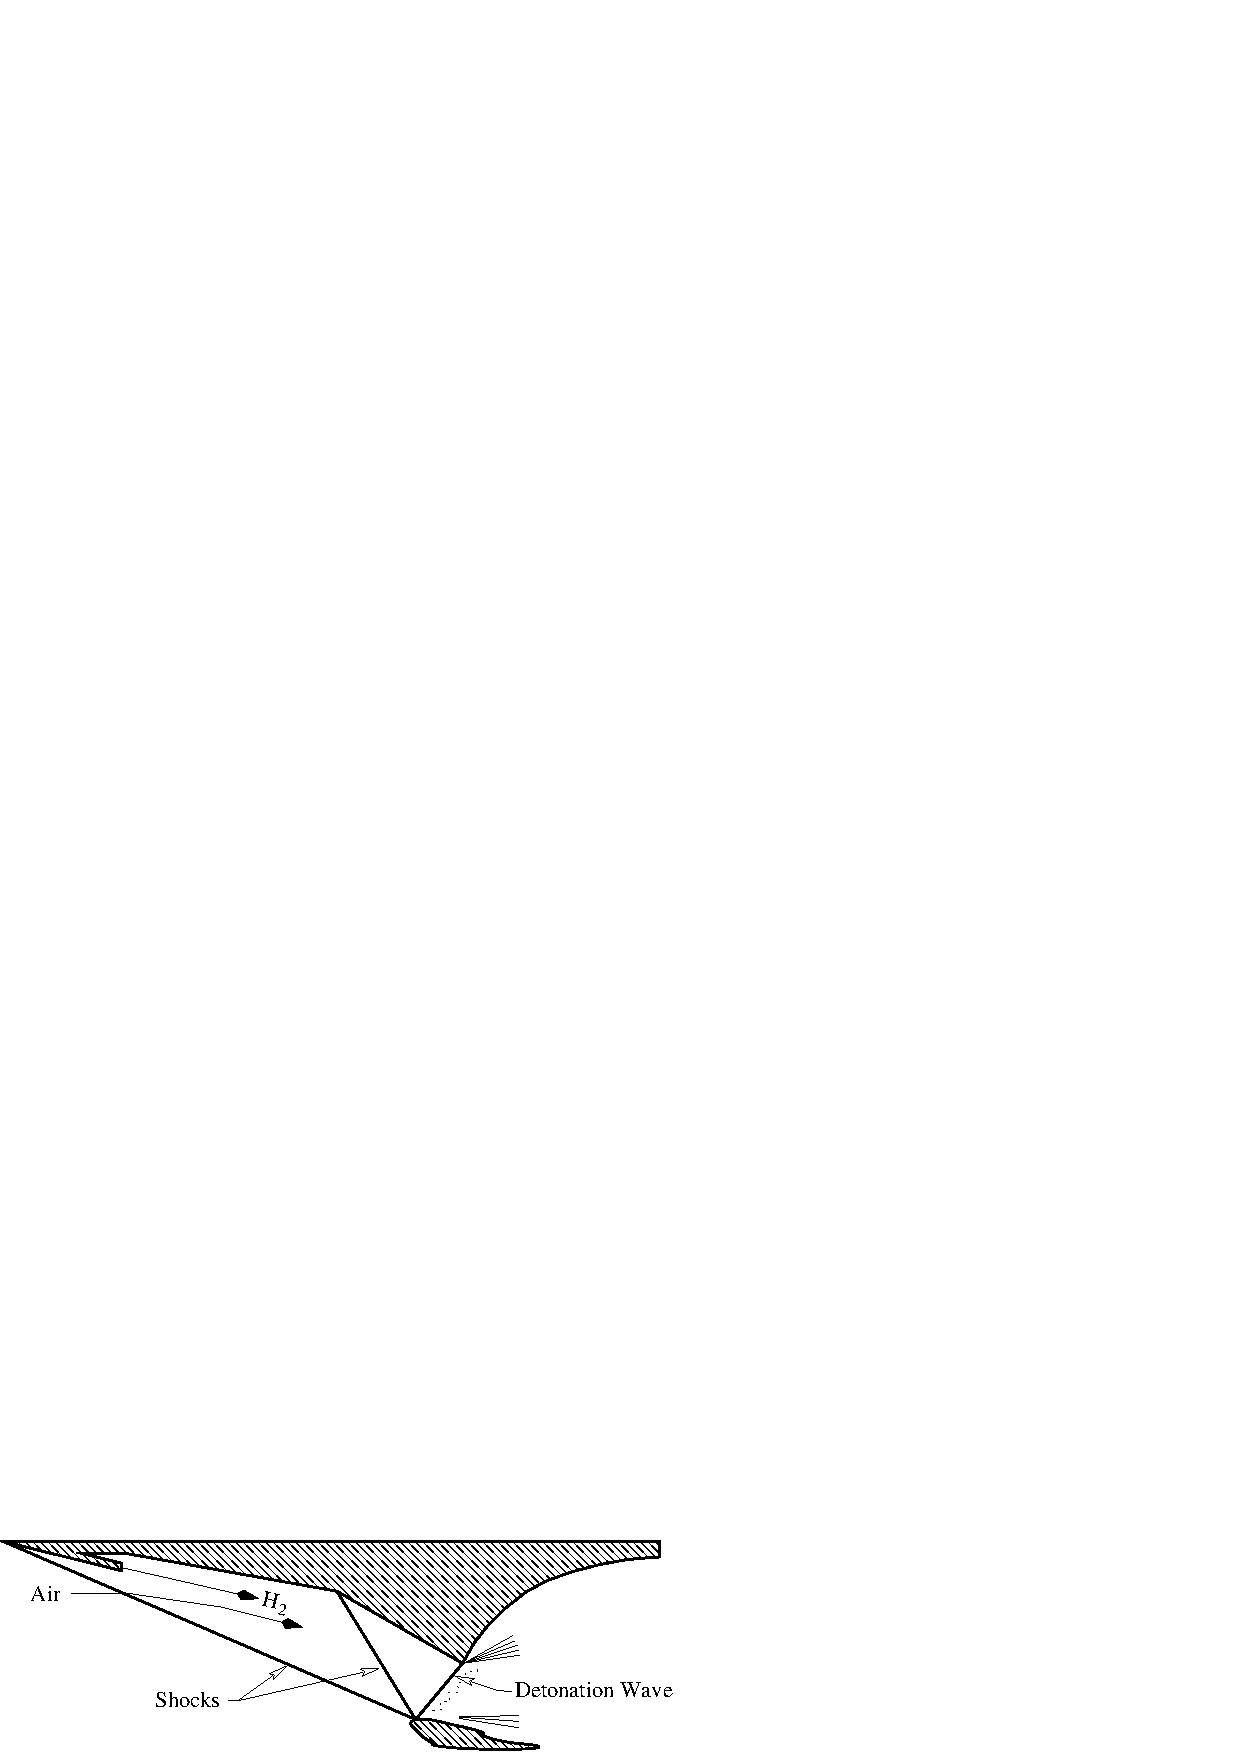
\includegraphics[width=4.0\lengthfigure]{fig1/shcramjet.pdf}
   \caption{External compression shcramjet schematic.}
   \label{fig:shcramjet}
\end{figure}
%



\section{The \emph{sh}ock-induced \emph{c}ombustion \emph{ramjet} (shcramjet)}


First proposed by Roy \cite{misc:1946:roy}, an alternate hypersonic propulsion concept
that aims at increasing the fuel
efficiency and thrust of the scramjet is the oblique detonation wave ramjet, also
referred to as the \emph{sh}ock-induced \emph{c}ombustion \emph{ramjet} (shcramjet)
\cite{aiaabook:2001:sislian,nasa:2000:jones}, as shown
in Figure \ref{fig:shcramjet}.  The massive
combustion chamber is avoided by burning the fuel/air mixture through a thin detonation
wave, with the fuel injected  in the inlet near the leading edge of the vehicle. This
reduces the weight of the engine and takes full advantage of the typically long inlets
found at hypervelocities.

Preliminary predictions of the performance of the shcramjet were
performed through
simplified one-dimensional analyses (see Sargeant and Gross \cite{misc:1959:sargeant}
or Dunlap \etal\ \cite{misc:1978:dunlap}). More detailed analytical
models ensued by Townend \cite{misc:1970:townend},
Morrison \cite{nasa:1978:morrison,nasa:1980:morrison},
and Ostrander \etal\ \cite{aiaaconf:1987:ostrander} to
assess the on-design and even off-design performance of the flight vehicle.
Later followed inviscid simulations of planar and axisymmetric
shcramjets by Sislian \etal\ using numerical methods based on exact and approximate
Riemann solvers
\cite{aiaaconf:1989:sislian,aiaaconf:1992:atamanchuk} also including
the non-equilibrium chemical kinetics equations for hydrogen/air combustion
\cite{jpp:1998:dudebout}.
The results obtained through the numerical studies confirm the encouraging
performance of the shcramjet found in previous analytical
work: (i) the shcramjet is seen to perform better than
a scramjet at high flight Mach number, and (ii) the shcramjet delivers a
fuel specific impulse superior to that of a rocket
up to a flight Mach number of 22 (see Ref.~\cite{jpp:1998:dudebout}).


Besides neglecting viscous effects, all of the above-mentioned studies assume
that no premature ignition occurs prior to the detonation wave, and
that the fuel and air are mixed in stoichiometric proportions prior to the
detonation wave.
To the author's knowledge, the only published work outlining the effect of
incomplete fuel/air mixing on the shcramjet performance is
Ref.~\cite{jpp:2000:sislian}, where Sislian \etal\ 
assess the impact of incomplete mixing on the net thrust by fixing
a non-uniform equivalence ratio distribution at the inlet entrance. It is observed that
an equivalence ratio distribution varying from $\phi \approx 2.4$ near the wall
to $\phi\approx 0.02$ in the freestream decreases the fuel specific impulse
by as much as $40\%$ in the flight Mach number range $9 \leq {\rm M}_{\rm flight} \leq 24$.
Due to the high sensitivity of the thrust of the shcramjet to incomplete fuel/air mixing,
achieving adequate fuel/air mixing in the inlet while preventing premature
ignition is one of the main technical challenges that needs to be
resolved to establish the shcramjet as a viable hypersonic airbreathing
flight vehicle.


%
\begin{SCfigure}
   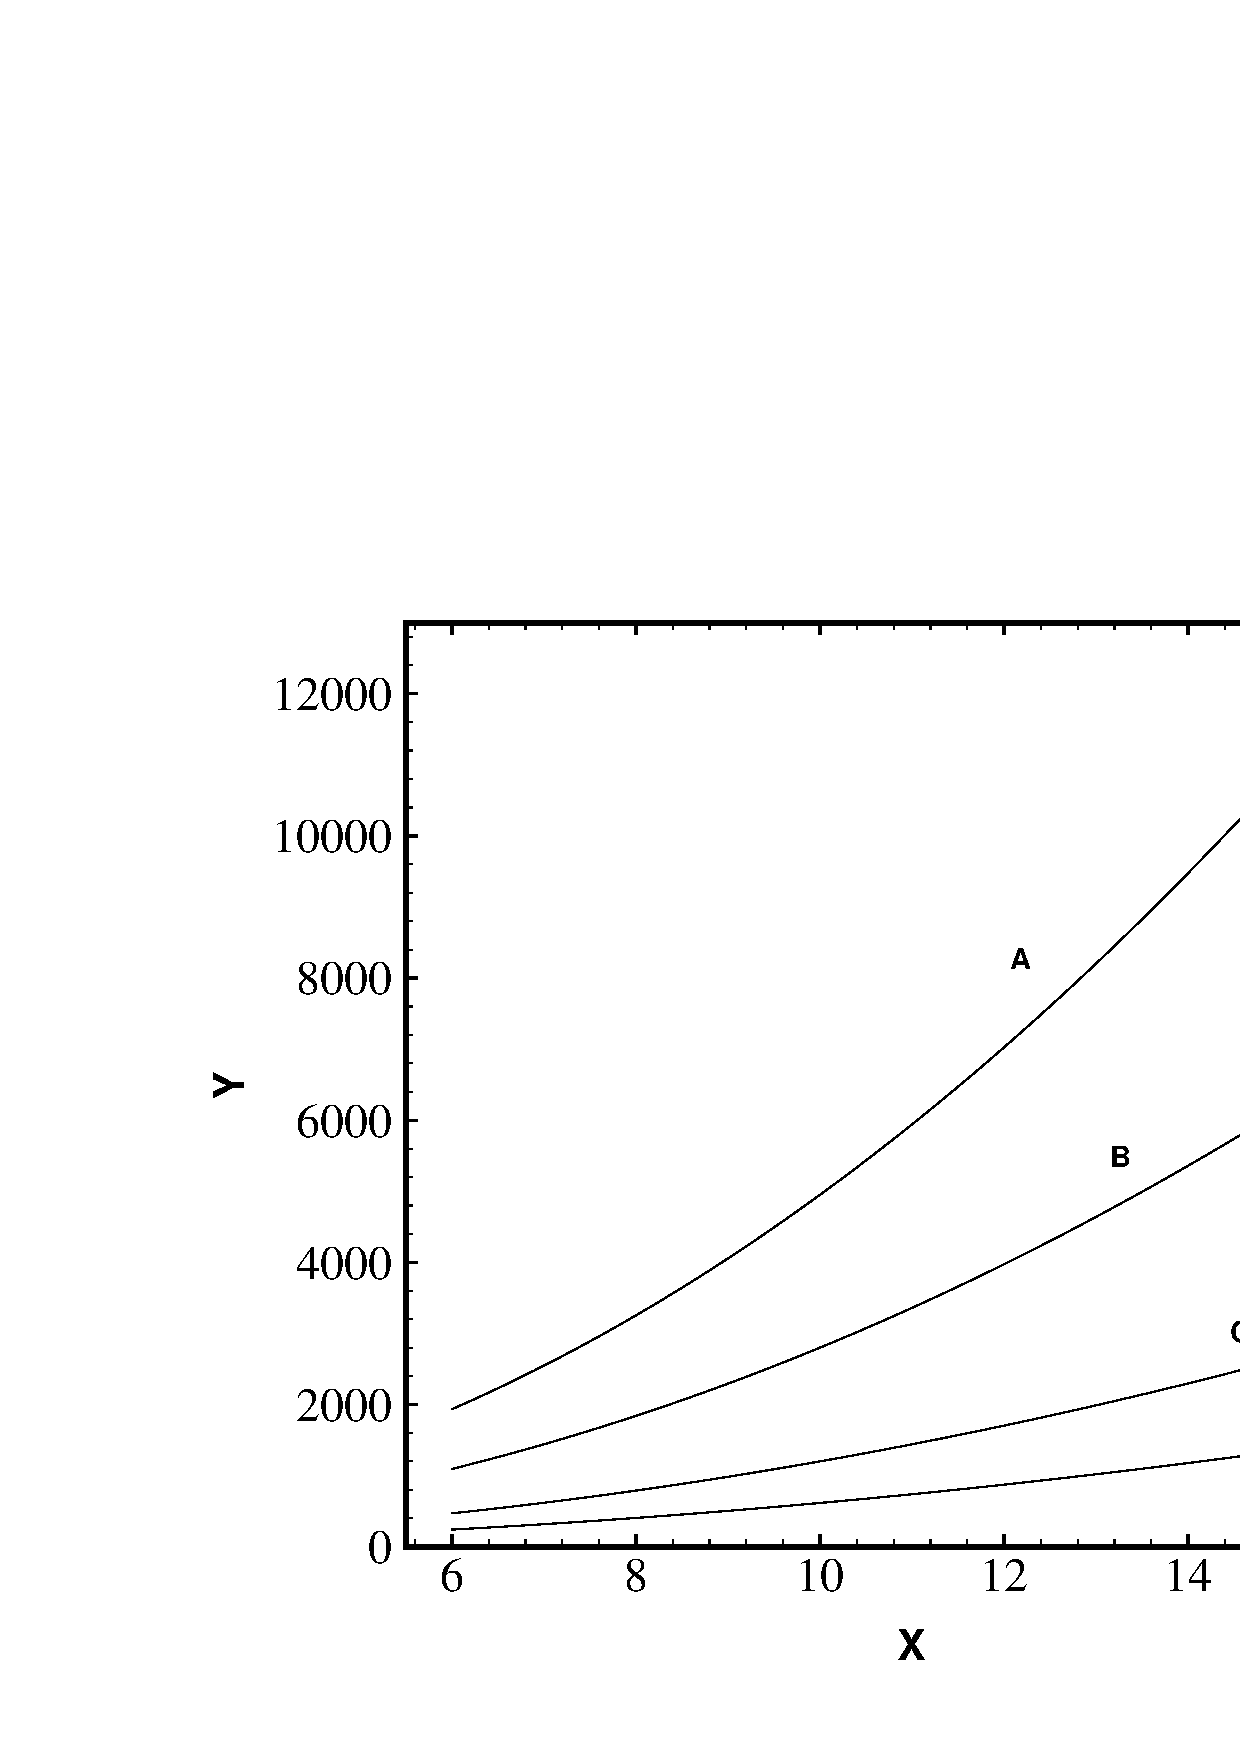
\includegraphics[width=3.8\lengthfigure]{fig1/combustor_entrance.pdf}
   \caption{Temperature at the combustor entrance versus the flight Mach
            number, assuming the ambient air temperature is 240~K, $\gamma=1.4$,
            and the deceleration process is isentropic.}
   \label{fig:combustor_entrance}
\end{SCfigure}
%


\section{Fuel/air mixing at hypervelocities}



Besides preventing premature ignition, it is desirable for
fuel injection in a hypersonic vehicle to be such that
most of the thrust due to the momentum
of the fuel is recovered by injecting the fuel in the same
direction as the surrounding freestream
(see Refs.~\cite{aiaa:1966:rubins,misc:1970:townend,
nasa:1978:morrison,nasa:1980:morrison}).
The need to inject fuel parallel to the surrounding freestream
direction is balanced by the need of adequate
fuel penetration in the incoming air while avoiding hard-to-cool intrusive parts.
This prompted the development of near-parallel
mixing configurations aimed at enhanced fuel penetration
and fuel/air contact surface stretching (see a recent review in
Ref.~\cite{misc:1995:gutmark} and other mixing strategies in
Refs.~\cite{jpp:1995:bushnell} and \cite{jpp:1994:bogdanoff}).


\subsection{Fuel pre-injection in scramjet inlets}


There has been a recent interest in pre-mixing the fuel with the air
upstream of the combustor to improve the mixing and burning performance  of
scramjets. Vasilev \etal\ \cite{aiaa:1994:vasilev} numerically investigate
on the fuel/air mixing in a Mach 8 inlet by means of an injector structurally detached
from the engine and placed well upstream of the inlet.
At the inlet exit,
a mixing completeness of as much as 0.6 to 0.7 is achieved without significant
stagnation pressure losses.
As a means to improve the efficiency of the heat release in scramjet combustors,
Segal \etal\ \cite{aiaa:2000:livingston,jpp:2001:owens} consider liquid
fuel pre-injection in the inlet, upstream of the combustor. They
experimentally investigate on the normal injection of
liquid fuel JP-10 behind thin pylons in a  Mach 1.6 and Mach 3.5
incoming air flow. The experimental results are representative of fuel injection
in the inlet
of a  scramjet operating in the lower end of the hypersonic flight regime,
where the high enthalpy incoming air flow interacts with the lower-speed fuel,
hence helping the process of liquid droplet breakup.
The use of pylons to inject gaseous hydrocarbon in a Mach 6--8
scramjet inlet is further investigated numerically by Guoskov \etal\
\cite{jpp:2001:guoskov}
who report a fuel-based mixing efficiency of 0.95 to 0.98 for
a global equivalence ratio varying between 0.3 and 0.7 respectively.
Both the experimental results by Segal \etal\ and the numerical results
by Guoskov \etal\ show that the pylons contribute
significantly to lift the liquid from the
injection surface, thus avoiding fuel in the boundary layer and potential
flashback.

%
\begin{figure}[!b]
   \center
   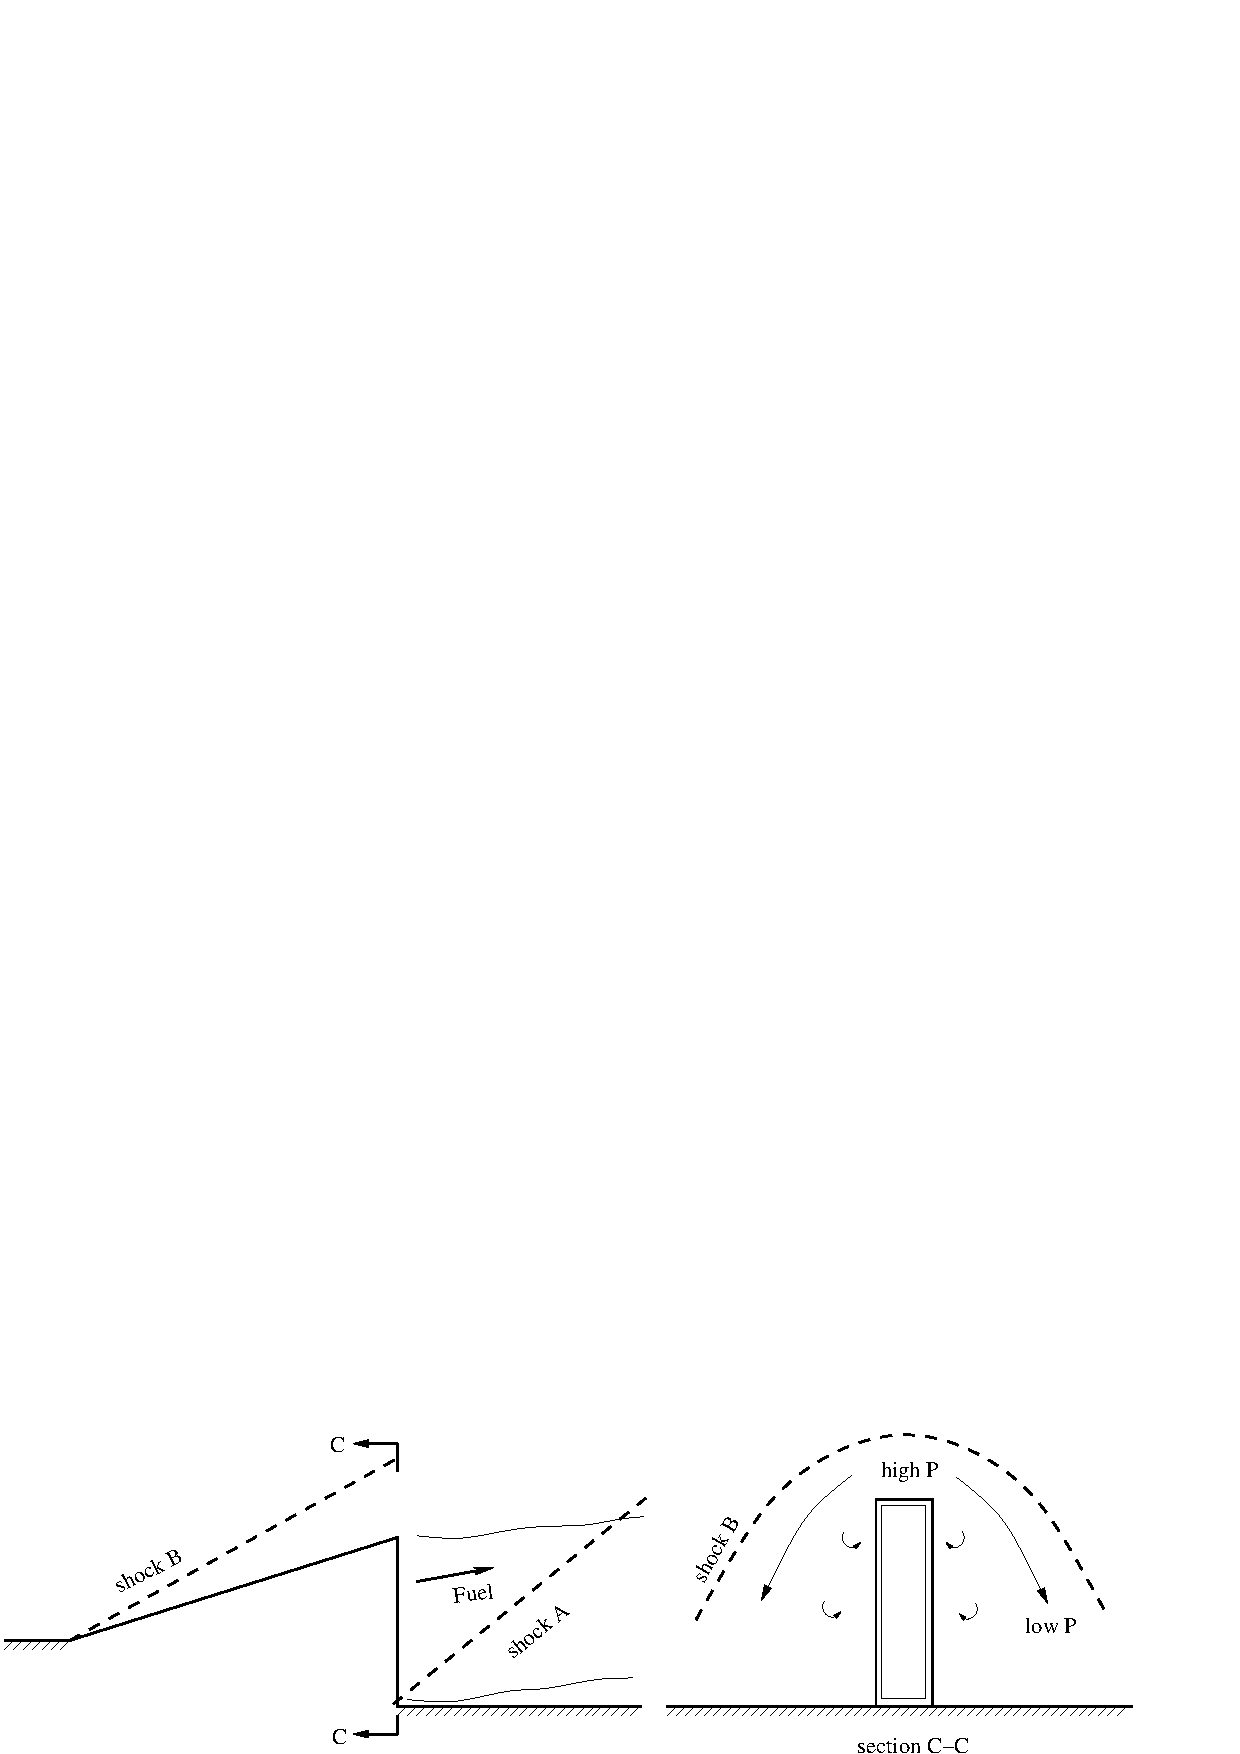
\includegraphics[width=4.6\lengthfigure]{fig1/ramp.pdf}
   \caption{Wall-mounted ramp injector schematic.}
   \label{fig:ramp-schema}
\end{figure}
%




\subsection{Choice of turbulence model}

Simple algebraic turbulence models (Cebeci-Smith and Baldwin-Lomax) were used
in almost all previous turbulent hypervelocity fuel/air mixing studies, with the
exception of a few \cite{aiaa:1998:lee,aiaaconf:1995:scherrer,jpp:1997:baurle}  where
``universal'' two-equation $k\epsilon$, $k\omega$ or $q\omega$ turbulence models were
considered. Also, the numerical investigations of inlet mixing reported so far
\cite{aiaa:1994:vasilev,jpp:2001:guoskov}
are limited to one-equation turbulence models without additional corrections
for compressibility effects.
In the present work, the Favre-averaged Navier-Stokes equations (FANS) are
closed by the low-Reynolds number $k\omega$ two-equation
turbulence model of Wilcox \cite{aiaa:1988:wilcox}. Despite its notable sensitivity
to the freestream conditions, the $k\omega$ model is preferred
to the $k\epsilon$ model due to its capability at solving
accurately the laminar sublayer of the turbulent boundary layer without the addition
of low-Reynolds number source terms \cite{aiaa:1988:wilcox}.
Aside from their inelegance, low-Reynolds
number source terms increase the stiffness of the governing equations and
require more grid points to be resolved properly. Further, the $k\epsilon$ model does
not predict correctly the growth of the boundary layer under an adverse pressure
gradient \cite{book:1994:wilcox}, a situation likely to occur in the inlet.
Wall functions are not used in the present study
as their accuracy is questionable in regions of
separated flow, which are present in the vicinity of the cantilevered ramp injector
and possibly in the vicinity of shock~/~boundary-layer interactions occurring
in the inlet. It is noted that improvements to the low-Reynolds number
Wilcox $k\omega$ model have been proposed recently by Menter \cite{nasa:1992:menter}
and later by Wilcox \cite{book:1998:wilcox}, in order to reduce the sensitivity of the $k\omega$
model to the freestream value of $\omega$. While showing great promise, the improved $k\omega$
models have not yet been validated as thoroughly in the literature as the low-Reynolds
number Wilcox $k\omega$ model, and are hence not considered for this study.

Among the various existing
compressibility corrections \cite{nasa:1978:sislian,thesis:1996:krishnamurty,
nasa:1994:coakley}, only the ``dilatational dissipation'' correction
\cite{misc:1990:zeman,jfm:1991:sarkar,aiaa:1992:wilcox} is retained in the
present investigation, due to a lack of experimental data justifying the presence of
other corrections. The use of the dilatational dissipation is particularly important
to predict the shcramjet inlet flowfield accurately due to the generally
high convective Mach number
in use. At a high convective Mach number,
compressibility effects are observed through experiments to restrict the growth
of the shear layer considerably \cite{jfm:1988:papamoschou,aiaabook:1991:dimotakis}.
This trend is not predicted correctly by the baseline $k\omega$ model and
a dilatational dissipation correction term needs to be introduced in the turbulence
kinetic energy equation to account for this compressibility effect. The dilatational
dissipation corrections proposed by Zeman \cite{misc:1990:zeman}
and by Sarkar \etal\ \cite{jfm:1991:sarkar} are applicable only to high
Reynolds number regions, and not in the laminar sublayer of the turbulent
boundary layer, for instance. Hence, the Sarkar and Zeman corrections are not
used for the mixing problems presented here as they result in an underprediction of
the wall shear
stress at the high flow Mach numbers typical of the shcramjet inlet. Instead,
the dilatational dissipation correction
of Wilcox \cite{aiaa:1992:wilcox} is preferred as it is shown not to alter the
shear stress over a flat plate up to a freestream Mach number of 6,
when used in conjunction with the $k\omega$ model.


\subsection{Discretization of the convection derivative}

Contrarily to the discretization of the diffusion terms which can
be accomplished through centered finite-difference stencils, the
discretization of the convection terms is problematic
(see Ch.~5 in Ref.~\cite{book:1980:patankar}).
A successful approach at discretizing the convection derivative is
through upwinding, as first proposed by Courant \etal\ \cite{misc:1952:courant}
for the solution of a scalar advection equation.
For the gas dynamics equations, the upwinded method is generalized by
Godunov \cite{misc:1959:godunov}, through the exact solution of a fictitious
Riemann problem midway between nodes. A simpler, linearized approximate Riemann
solver based on eigenvalue splitting is later proposed by
Roe \cite{jcp:1981:roe}. The Roe scheme has
the property of reverting to a first-order upwind stencil in case of locally
supersonic flow, and of reverting to a centered finite difference scheme with
matrix dissipation when the local velocity is much smaller than sonic.
Probably due to its relative
ease of extension to different governing equations, and its ease of linearization
when used in conjunction with an implicit scheme, the Roe scheme has
become one of the preferred Riemann-solver-type method
for compressible flow. Yee \etal\ \cite{jcp:1990:yee} extend the Roe method to
second-order accuracy
while retaining the original monoticity of the first-order method by the use
of flux limiters, resulting in increased accuracy for many flowfields. The
latter is the discretization method chosen for this study, and is
referred to hereafter as the Yee-Roe scheme. The Yee-Roe
scheme is here applied in coupled form to all transport equations, including the turbulence
kinetic energy, the specific dissipation rate of the turbulence kinetic energy,
the continuity, the momentum, and the energy
transport equations. The eigenstructure of the Roe flux Jacobian for the FANS
equations is presented.


\subsection{Pseudotime stepping}

An implicit strategy is here chosen to advance the solution in pseudotime
to steady-state, in order to relieve the constraints on the pseudotime step size
imposed by the viscous terms in flow regions where the grid spacing is small
(such as in the laminar sublayer of the turbulent boundary layer for instance).
To minimize storage requirements and the inversion effort,
a block-implicit approximate-factorization (AF) algorithm
\cite{jcp:1977:briley, aiaa:1978:beam} is used.
The convection terms are linearized assuming a frozen Roe Jacobian, while
the viscous terms are linearized following a strategy outlined
in Chang and Merkle \cite{jcp:1989:chang}.
While relatively dated (the scalar approximate-factorization
algorithm dates back almost 50 years and the block-implicit version was
first proposed in the late 1970's), block-implicit AF
is still at the heart
of many numerical methods solving the Euler or Navier-Stokes equations in the
hypersonic range (see Refs.~\cite{aiaaconf:1997:maccormack,cf:2001:maccormack}
for instance). Despite having the potential to significantly accelerate the
convergence of the baseline block implicit AF method,
Newton-Krylov and multigrid methods are rare in
present day codes aimed at solving hypersonic viscous flows. Additional difficulties
in the hypersonic range originate from strongly non-linear phenomena (such as
shock waves and chemical reactions) that hamper the performance of multigrid,
although recent advancements shed some hope that this can be remedied,
at least for certain flowfields \cite{jcp:2001:gerlinger}.


\subsubsection{Convergence acceleration through space-marching}

There is little doubt that the most efficient way to solve
supersonic or hypersonic flow with no streamwise ellipticity is
through a space-marching method, as numerous extremely efficient
marching methods developed over the years can attest (see for example Refs.
\cite{aiaaconf:1978:vigneron,aiaaconf:1986:lawrence,aiaaconf:1988:tannehill,
cf:1997:dambrosio,cf:1998:miller}). The Navier-Stokes equations at supersonic
speeds do, however, exhibit some ellipticity in the marching direction through
the streamwise viscous terms and the subsonic layer of the boundary layer,
and it is necessary for a space-marching method to ignore these mechanisms by
solving a reduced set of the original equations of motion, such as
the parabolized Navier-Stokes equations (PNS). The PNS are defined here as
the equation set obtained
from the Navier-Stokes equations by neglecting all viscous terms in the
streamwise direction and by modifying the streamwise momentum equation to
prevent any pressure
disturbance from traveling upstream, using characteristics splitting or pressure
splitting as suggested by Vigneron \etal\ \cite{aiaaconf:1978:vigneron}.
The applicability of the space-marching methods is
limited to flows with negligible streamwise ellipticity, hence preventing their
deployment to many practical flowfields.


\subsubsection{Difficulties originating from large streamwise-separated regions}

The need to tackle streamwise ellipticity prompted the development
of the ``global iteration'' space-marching methods in which
a sweep is performed several times on the entire computational
domain to permit the upstream propagation of information
(see Ref.~\cite{aiaa:2000:miller} for a detailed review).
These schemes are characterized, compared to the pseudotime marching schemes,
by a smaller memory requirement due to the storage
of temporary variables in one marching plane only and by
enhanced wave propagation mechanism in the streamwise
direction. The reduced Navier-Stokes (RNS) equations, which are derived from
the Navier-Stokes equations by ignoring all streamwise diffusion terms but
not altering the momentum convection terms,
are usually solved in this manner leading to fast convergence of subsonic/supersonic
streamwise unseparated flows \cite{aiaa:1988:power,jcp:1989:chang,aiaa:2000:yamaleev}
and even of viscous/inviscid interactions creating streamwise separation
\cite{cf:1983:rubin,aiaa:1986:barnett}. In a similar vein,
Bardina \cite{aiaaconf:1994:bardina} shows that significant reduction in work
is achievable by the use of  global marching sweeps to solve the full
Navier-Stokes equations for high-speed flows. However, if not limited to some
predetermined zones of the computational domain, the global iteration
approach loses some performance when solving large reverse flow regions,
as the number of sweeps can become excessive due to its dependence
on the size in streamwise grid lines of the separation bubble.
Further, some computing might be inefficiently
allocated to the nodes downstream of the separation bubble, \emph{prior} to its
convergence. These deficiencies can be remedied by using a space-marching
scheme solving the PNS equations until an elliptic/reverse flow region is
encountered, then switching to a global iteration RNS method (or FANS)
for the length of the
elliptic region, iterating until convergence is reached, and pursuing with
the marching PNS scheme (see Miller \etal\ \cite{aiaa:2000:miller} for instance).
However, such a strategy forces the solution of the PNS equations in certain
regions of the flowfield for which the PNS assumption might induce
appreciable errors. The accuracy of the final solution is hence strongly
dependent on the ability of the method at predicting correctly which
regions of the flowfield can be accurately predicted with the PNS equations,
and which regions require the use of the RNS (or FANS) equations.


\subsubsection{The domain rollover method}

In Ref.\ \cite{thesis:1997:underwood}, Underwood presents
a technique based on domain decomposition which is
aimed at improving the generality of the above-outlined PNS
methods with embedded elliptic solvers. The technique
is dubbed ``domain rollover'' and can be summarized as follows.
Prior to the iterative process, the physical domain is divided into a
series of subdomains in the streamwise
direction. Then, the FANS equations are iterated in
pseudotime on a solution domain which is
composed of a certain number of adjacent subdomains (the number of subdomains
being user-specified). When the residual
in the upstream subdomain part of the solution domain falls below a user-specified
convergence threshold, the solution domain advances by one subdomain in the
streamwise direction. To correctly capture regions of streamwise ellipticity,
it must hence be ensured before starting the iterative process that each
subdomain is large enough to contain the streamwise-elliptic regions
that are expected to form in its interior. This is necessary due to the lack
of ``streamwise ellipticity sensors'' at the upstream and downstream
boundaries of the solution domain. The lack of sensors prevents a locally elliptic
region to outgrow the solution domain boundaries. Therefore,
similarly to the PNS methods with embedded elliptic solvers,
the success of the domain rollover method at predicting accurately flowfields
including streamwise-elliptic regions depends on the ability of the user
at predicting \apriori\ the location and size of the zones of streamwise ellipticity.








\subsubsection{The active domain method}

Recently, a novel approach at solving inviscid supersonic flow with embedded
subsonic regions has been proposed \cite{aiaa:1997:nakahashi}. The method,
named ``active domain'', consists of performing pseudotime iterations
on a small band-like computational domain that advances in the streamwise direction
every time the residual of the active domain near the upstream
boundary falls below a user-defined threshold.
Using sensors based on the streamwise component of the Mach number,
the active domain boundaries automatically surround any
locally subsonic region, on which sufficient iterations are performed to reach
steady-state. When the residual inside the subsonic region decreases below
the user-defined threshold, the active domain advances past the subsonic region
further downstream. By marching in the streamwise direction, the active domain
results in a decrease
in work of up to 10 times compared to standard pseudotime marching methods
for several inviscid problems. However, the ability of the active domain at solving accurately a
streamwise elliptic region is limited by the accuracy of the sensor responsible for the
upstream movement of the upstream boundary of the active domain. Extension
of the active domain method to viscous flow is hampered by the
difficulty of formulating a streamwise ellipticity sensor that captures
all significant upstream propagating waves while restricting the size of
the active domain to a minimum. Success has been reported in solving
viscous flow without streamwise separation by maintaining the active domain
width equal to the height of the boundary layer \cite{aiaaconf:1999:morino}.
However, to the author's knowledge, the active domain method has not yet been extended
to streamwise separated flows.



\subsubsection{A new convergence acceleration technique}

This thesis proposes an alternate form of the active domain method,
named the ``marching window'' algorithm, that can be used to solve the FANS
equations for problems including streamwise separated flows. Similarly to the
active domain, the marching window
performs localized pseudotime stepping on a subdomain
composed of a sequence of streamwise planes. The width of the marching window
decreases to only a few planes in regions of quasihyperbolic flow
and increases to the size of the streamwise-elliptic region when encountered.
However, in sharp contrast to the active domain algorithm (and also to the domain
rollover algorithm), the marching window is
strictly a convergence acceleration technique as it guarantees the residual of
all nodes to be below the user-defined threshold when convergence is attained.
This is accomplished by keeping the residual upstream of the marching
window subdomain updated at all times, and by positioning the upstream boundary
such that the residual of all nodes upstream is below the user-defined threshold.
This results in an algorithm that captures all upstream
propagating waves affecting the residual significantly. The upstream
propagating waves can originate from (but are not necessarily limited to) large subsonic
pockets, streamwise separation, streamwise viscous fluxes, or the flux limiters in
the streamwise convection flux derivative, for instance. Further,
to enhance the performance of the algorithm,
a sensor based on the Vigneron splitting \cite{aiaaconf:1978:vigneron}
is developed to advance the downstream boundary
when significant streamwise ellipticity is detected.


To assess the performance of the marching window, several numerical experiments are
presented in Chapter~\ref{chapter:numerical_method}
ranging from the inviscid solution
of a supersonic inlet with a blunt leading edge to turbulent shock boundary layer interactions
with considerable streamwise flow separation solved with the FANS
equations closed by the $k\omega$ turbulence
model of Wilcox \cite{aiaa:1988:wilcox}. A time accurate turbulent flow field using
dual time stepping is also investigated. In all cases, a comparison between the
marching window cycle, the active domain cycle (for the inviscid case only),
and the standard pseudotime marching cycle
is made on the basis of CPU time, effective iterations, and storage.


  % introduction
% add a chapter about the governing equations (the physical model)
  \begin{chapterquote}
 ``It is amusing to note that fluid equations were developed originally to
 simplify the discrete equations of individual particle dynamics. Now we must
 reformulate the continuum problem to solve equations for finite volumes of material.''
 \quoteauthor{Elaine Oran and Jay Boris}
\end{chapterquote}

\chapter{Numerical method}
\label{chapter:numerical_method}

\section{Overview}

This chapter outlines the numerical method used to solve the FANS governing equations
shown in the previous chapter. The ``overlines'' and
``tildes'' used to denote time-averaged properties in the previous chapter
are dropped here for convenience. All derivatives appearing in the diffusion,
source, and metrics terms are approximated using centered second-order accurate
finite-difference stencils, while the convection derivative is modeled through
the Yee-Roe \cite{book:1998:laney} scheme. A block implicit approximate factorization
algorithm solves the discretized form of the residual to steady-state with
the use of a CFL-based local pseudotime step. Also, a novel convergence acceleration
algorithm based on domain decomposition is presented, named the marching window.
The marching window is shown to decrease the work needed to
reach steady-state by $\sim 10$ times for several viscous hypersonic problems
involving large streamwise recirculation regions.



\section{Exact form of the residual}

The residual of the full Navier-Stokes equations
can be expressed in generalized coordinates in tensor
form for any number of dimensions as
%
\begin{equation}
 \frameeqn{
 R=
     \sum_{i=1}^{\nd}
      \left[ \frac{\partial {F_i}}{\partial X_i}
            - \sum_{j=1}^{\nd} \frac{\partial }{\partial X_i}
             \left( K_{ij} \frac{\partial G}{\partial X_j}\right) \right]
     -S
 }~,
  \label{eqn:residual}
\end{equation}
%
where the minimization of $R$ is sought and where $d$ refers to the number of dimensions.
Due to the non-linearity of the system of equations,
a fictitious unsteady term ${\partial Q}/{\partial \pseudot}$
is necessary to obtain the right physical root from a given set of initial conditions,
\ie
%
\begin{equation}
 \frac{\partial Q}{\partial \pseudot} =-R \, .
\end{equation}
%
Even though the numerical methods outlined in this chapter
(including the spatial and temporal discretization along with
the pseudotime stepping schemes) are
not linked to some governing equations in particular,
this study focuses on the Favre averaged Navier-Stokes equations (FANS)
closed by the Wilcox $k\omega$ model \cite{aiaa:1988:wilcox} shown in the
previous chapter.
The vectors $Q$, $F$, $G$ and the conductivity matrix $K$ part
of the RHS of Eq.~(\ref{eqn:residual}) can be obtained from ...
and ...
The source term $S$ is composed of the sum of
a modification to the baseline Wilcox $k\omega$ source terms outlined
in Eq.~... with the dilational dissipation $\epsilon_d$
and an unsteady source term,
%
\begin{equation}
  S=
  \frac{1}{J} \left[
  \begin{array}{c}
    \vdots \alb
    0 \alb
    P_k- \rho k \omega  -\rho \epsilon_d \alb
    \bigfrac{\omega}{\widetilde{k}}\left(
      {\mfc\frac{5}{9}} P_k - {\mfc\frac{5}{6}} \rho k \omega
      + \rho \epsilon_d
    \right)
  \end{array}
  \right]
  - \frac{\partial Q}{\partial t} \, ,
\end{equation}
%
where the turbulent kinetic energy production term was defined previously
in Eq.~...
It is noted that in the Wilcox $k\omega$ model, $\widetilde{k}$ is
set simply to $k$ which in the freestream is set to a small
value to prevent a division by zero. We prefer, however, to specify
$k=0$  in the freestream and, in order to prevent a division by zero
in the dissipation rate source term, to define $\widetilde{k}$ as
%
\begin{equation}
  \widetilde{k}={\rm max}\left[ k ~,~~\min \left(k_{\rm div}~,
                 ~~\frac{\omega \mu} {\rho}\right)\right] \, ,
  \label{eqn:ktilde}
\end{equation}
%
with $k_{\rm div}$ a user-specified constant which is generally set lower than
one tenth of the maximum value of $k$ throughout the boundary layer. This is
verified numerically not to affect the laminar sublayer
but to improve the robustness and efficiency of the integration significantly.
The minimum between $k_{\rm div}$ and $\omega \mu / \rho$ is taken so that a
clipping occurs \emph{only} in non-turbulent flow regions in which an accurate
representation of $\omega$ does not affect the accuracy of the flowfield.




\section{Discretized form of the residual}

The discretization of all terms in the residual is now presented.
By referring to the discretized form of the derivatives along the
$X_i$ coordinate by $\delta_{X_i}$, the discretized residual
$R_\Delta$ can be written as
%
\begin{equation}
\frameeqn{
R_\Delta = \sum_{i=1}^{\nd}  \left[
   \delta_{X_i} F_i -
       \sum_{j=1}^{\nd}
      \delta_{X_i} \left( K_{ij} \delta_{X_j} G\right)
   \right] -S_\Delta
}~,
\label{eqn:resdelta}
\end{equation}
%



\subsection{Diffusion terms}

The
use of tensor form in writing the governing equations in curvilinear
coordinates shown in Eq.~(\ref{eqn:residual}), along with the unique compact
$K_{ij}$ matrix described in Eq.~(...), simplify greatly the discretization
and practical implementation of the viscous terms: less than 100 lines of code are
needed to implement the viscous contribution of the residual for all $d \in [1,~2,~3]$.
Using second-order accurate
centered finite difference stencils, the discretization of the viscous terms,
with $i=j$, corresponds to
%
\begin{equation}
 \frameeqn{
\left[ \delta_{X_i} \left( {K_{ii}}\delta_{X_i} G \right) \right]^{X_i}
 =K_{ii}^{X_i+\frac{1}{2}} \left( G^{X_i+1}-G^{X_i} \right)-
  K_{ii}^{X_i-\frac{1}{2}} \left( G^{X_i}-G^{X_i-1} \right)
 }~,
\end{equation}
%
and, with $i \neq j$, corresponds to,
%
\begin{equation}
 \frameeqn{
 \begin{array}{l}
   \left[ \delta_{X_i}\left( K_{ij}\delta_{X_j} G \right) \right]^{X_i,X_j}\alb
   \begin{array}{rl}
 ~=\!\!&\!\!\! \frac{1}{4} K_{ij}^{X_i+\frac{1}{2},X_j} \left(G^{X_i,X_j+1}+G^{X_i+1,X_j+1} -G^{X_i,X_j-1}-G^{X_i+1,X_j-1}  \right) \alb
 ~-\!\!&\!\!\! \frac{1}{4} K_{ij}^{X_i-\frac{1}{2},X_j} \left(G^{X_i-1,X_j+1}+G^{X_i,X_j+1} -G^{X_i-1,X_j-1}-G^{X_i,X_j-1}  \right)
   \end{array}
 \end{array}
 }~,
\end{equation}
%
where $K^{X_i+\frac{1}{2}}$ midway between nodes is
taken as half the value of $K^{X_i+1}$ and $K^{X_i}$ for example.



\subsection{Convection terms: Yee-Roe flux limited method}

The Yee-Roe flux-limited method here refers to the second-order extension
of the Roe scheme \cite{jcp:1981:roe} by
the Yee limiters applied to the characteristic variables \cite{jcp:1990:yee}.
The first-order accurate Roe scheme is itself a generalization to
a system of multiple equations of
the Courant upwinded scheme \cite{misc:1952:courant} for a scalar advection equation,
which can be written as
%
\begin{equation}
  a\frac{\partial q}{\partial X_i} \approx
  a \left\{
    \begin{array}{ll} q^{X_i+1}-q^{X_i} & ~~{\rm if}~a<0 \\
                      q^{X_i}-q^{X_i-1} & ~~{\rm otherwise,}\end{array}
\right.
\end{equation}
%
where the RHS corresponds exactly to
%
\begin{equation}
  \frac{1}{2} \left[
                         a q^{X_i+1}- a q^{X_i-1}
                       - |a| \left( q^{X_i+1} - q^{X_i} \right)
                       + |a| \left( q^{X_i} - q^{X_i-1} \right) \right]~.
\end{equation}
%
Roe extends the Courant \etal\ upwinded method to a system of equations through
an upwinded stencil based on the sign of the eigenvalues, namely
%
\begin{equation}
\left[ \delta_{X_i} F_i \right]^{X_i}=\frac{1}{2}\left[ F_{i}^{X_i+1}-F_{i}^{X_i-1}
          - \left[ \frac{L^{-1}_i |\lambda_i| M_i}{J} \right]^{X_i+\frac{1}{2}}
          + \left[ \frac{L^{-1}_i |\lambda_i| M_i}{J} \right]^{X_i-\frac{1}{2}} \right],
\end{equation}
%
where $|\lambda_i|$ and $L_i$ stand for the absolute value of the eigenvalues and
left eigenvectors of the
convective flux Jacobian  $A_i\equiv \partial F_i / \partial Q$
and where the characteristic variables vector $M_i$ corresponds to
%
\begin{equation}
 M_{i}^{X_i}=L_i^{X_i}\left( \left( JQ \right)^{X_i+\frac{1}{2}}
                      - \left(JQ\right)^{X_i-\frac{1}{2}} \right).
\end{equation}
%
All flow properties part
of the eigenvalues and and part of the left and right eigenvectors of the flux Jacobian
evaluated in-between nodes in Eq.~(\ref{eqn:deltaF}) are determined using Roe averaging
\cite{jcp:1981:roe},
such that the Roe scheme yields a first-order backward stencil in the case of
supersonic flow,
\ie\ $F_i^{X_i+1}-F_i^{X_i}=A_i^{X_i+\frac{1}{2}}(Q^{X_i+1}-Q^{X_i})$, which is
the same stencil yielded by the Godunov exact Riemann solver \cite{misc:1959:godunov}.
It is noted
that the Roe averaging outlined in Ref.~\cite{jcp:1981:roe} is applicable only
to a perfect gas, and would not yield a first-order backward difference in the
case of a calorically non-perfect gas, as used in this study. The extension of the
Roe average to a calorically non-perfect gas (as in Ref.~\cite{jcp:1989:liu}) is
achieved by constructing two flux Jacobian matrices (so-called homogeneous and
heterogeneous) from two different vectors of
conservative variables. We prefer not to follow this approach in this study,
and to use the Roe averaging at the interface, from which the flux Jacobian
is uniquely constructed from a single $Q$ vector. While this does not yield exactly
a first-order backward difference in the case of supersonic flow, experience
shows that the type of averaging used at the interface is not an issue to be particularly
concerned about, with simple arithmetic averaging commonly being used (see
for example Refs.~\cite{aiaaconf:1997:maccormack,cf:2001:maccormack}).
Yee \etal\ \cite{jcp:1990:yee} extend the Roe scheme to second-order accuracy
by determining the characteristic variables at the interface from a
limited second order stencil:
%
\begin{equation}
 \frameeqn{
\left[ \delta_{X_i} F_i \right]^{X_i}=\frac{1}{2}\left[ F_{i}^{X_i+1}-F_{i}^{X_i-1}
          - \left[ \frac{L^{-1}_i |\lambda_i| N_i}{J} \right]^{X_i+\frac{1}{2}}
          + \left[ \frac{L^{-1}_i |\lambda_i| N_i}{J} \right]^{X_i-\frac{1}{2}} \right]
}~,
\label{eqn:deltaF}
\end{equation}
%
\begin{equation}
{\rm with~~~} N_i^{X_i} = M^{X_i}_i-\minmod \left( M^{X_i-1}_i~,
                      ~~M^{X_i}_i~, ~~M^{X_i+1}_i\right).
\end{equation}
%
For the minmod limiter to be in pseudo control volume form, it is necessary
to ensure that all metric terms needed to construct the $N$ matrix at one cell
interface are measured at that particular interface.

A small positive value
can be added to the eigenvalues to fix the aphysical carbuncle phenomenon
originating from the Roe scheme when tackling certain problems, especially blunt
bodies. This is usually referred to as ``entropy correction'',
but is just a convenient way of adding artificial dissipation to
the flux discretization \cite{jcp:1997:batten} and can significantly
deteriorate the accuracy of the scheme in turbulent boundary layers (see for
example results obtained by Parent and Sislian \cite{aiaaconf:2001:parent}).
Unless otherwise indicated, no entropy correction term is used for the
problems presented herein.



\subsection{Source terms}

All partial derivatives of the discretized source term $S_\Delta$
are determined from second order accurate three-point stencils, except for the stencil
of the time derivative term, which is limited and is set to,
%
\begin{equation}
 \frameeqn{
 \begin{array}{r}
  \delta_t Q = \bigfrac{1}{\Delta t}
      \left[ Q^t-Q^{t-\Delta t}
             + \bigfrac{1}{2} \, \minmod \left( Q^t-Q^{t-\Delta t},~Q^{t-\Delta t}-Q^{t-2\Delta t} \right)
      \right.
  \alb
      \left.
             - \bigfrac{1}{2} \, \minmod \left(Q^t-Q^{t-\Delta t},~Q^{t-\Delta t}-Q^{t-2\Delta t},~Q^{t-2 \Delta t}-Q^{t-3\Delta t}\right)
      \right]
 \end{array}
 }~,
 \label{eqn:dQdt}
\end{equation}
%
where the minmod function returns the minimum of its arguments if the arguments
are all positive, the maximum if the arguments are all negative,
and zero if the arguments are of mixed signs. It is noted that the second
order contribution in Eq.~(\ref{eqn:dQdt}) is in non-conservative form,
but, to the authors' knowledge,  such is unavoidable if no future value
of $Q$ (at a time $t+\Delta t$) is included in the stencil and a
second-order accurate stencil
that results in no spurious oscillations is desired. The non-conservation of
the stencil is very weak and numerical tests indicate that Eq.~(\ref{eqn:dQdt})
is adequate.


\subsection{Eigenstructure of the convective flux Jacobian}

%
\begin{SCfigure}
   \fontsizefigure
   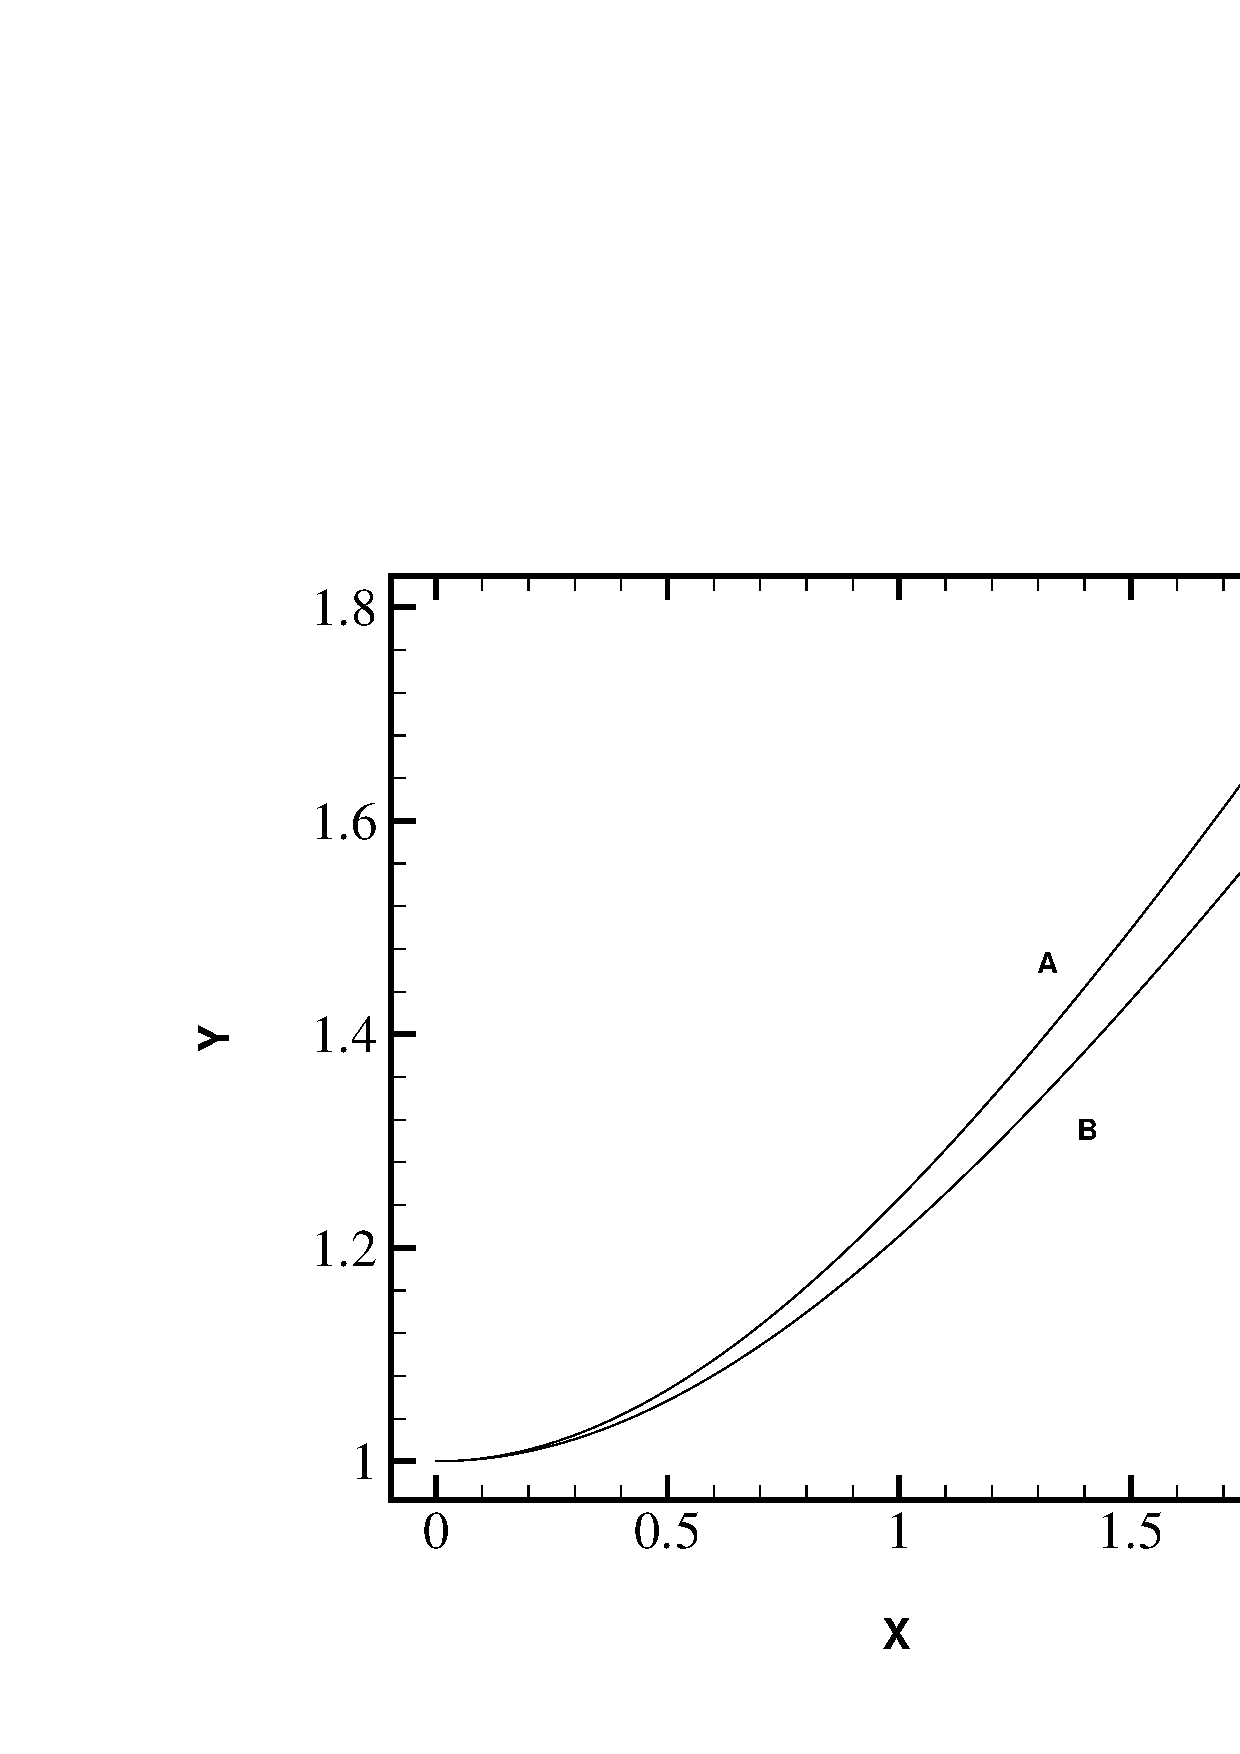
\includegraphics[width=3.36\lengthfigure]{fig3/ParentFig1.pdf}
\caption{Normalized speed of sound $\overline{a}=a/a_{k=0}$
         versus the turbulent Mach number $\Mt=\sqrt{2k}/a_{k=0}$,
         for a calorically perfect gas according to
         Eq.~(\ref{eqn:anorm}).}
\label{fig:anorm-Mturb}
\end{SCfigure}
%

Since the Roe scheme is used to discretize the convection derivatives,
the determination of the eigenstructure of the convective flux Jacobian
$A_i\equiv \partial F_i / \partial Q$ is needed.
It can be checked by substitution that the following definition of $\lambda_i$,
%
\begin{equation}
  \frameeqn{
 \lambda_i=
 \left[
   V_i,~~
   V_i,~~
   \rightarrow,~~
   V_i + a\widehat{X}_i,~~
   V_i - a\widehat{X}_i,~~
   V_i,~~
   V_i
 \right]^{\rm D}
 }~,
 \label{eqn:lambda}
\end{equation}
%
satisfies the necessary relationship ${\rm det}(A_i-w_i I)=0$ (with $w_i$ any element
on the diagonal of $\lambda_i$) and is hence a valid eigenvalue matrix.
Denoting the flow speed by $q$, the non-metric effective speed of sound is found to
be equal to
%
\begin{equation}
  a=\left( P_\rho + \frac{2}{3} k +P_{\rho E} \left( H-q^2-k\right) \right)^{\frac{1}{2}},
  \label{eqn:a}
\end{equation}
%
which as might be expected is a function of the
kinetic energy of turbulence, in contrast to the ``non-turbulent''
speed of sound (here denoted by $a_{k=0}$)
encountered in the eigenstructure of the convection terms of the molecular Navier-Stokes
equations. Dividing both sides of Eq.~(\ref{eqn:a}) by
$a_{k=0}$ and after some reformatting, the normalized speed of sound
can be shown to be equal to
%
\begin{equation}
  \overline{a} \equiv \frac{a}{a_{k=0}}= \left(1+\frac{P_{\rho E}+1}{3} \Mt^2\right)^{\frac{1}{2}},
  \label{eqn:anorm}
\end{equation}
%
where for a calorically perfect gas, $P_{\rho E}+1$ is equal to the ratio of the specific heats,
$\gamma$. Figure \ref{fig:anorm-Mturb} shows the relationship
between $\overline{a}$ and the turbulent Mach number for $\gamma=7/5$
and $\gamma=5/3$.
As the turbulent Mach number increases, its influence on $\overline{a}$
becomes more predominant due to the relative speed of the turbulent
vortices, with respect to the average vortex speed of displacement, gradually
overtaking the thermodynamic sound speed as the information propagation mechanism.
For a perfect or real gas, the derivatives of pressure with respect to the
mass-weighted total energy and density are equal to
%
\begin{equation}
  P_{\rho E}=\bigfrac{1}{\rho \bigfrac{\partial }{\partial P}e(P,\rho)}~~~{\rm and}~~~
  P_{\rho_k}=\left[-\mfd\frac{E-k-q^2}{\rho}- \mfd\frac{\partial e(P,\rho)}{\partial \rho_k} \right]
             \left/ \mfd\frac{\partial e(P,\rho)}{\partial P} \right.~,
\end{equation}
%
with $e$ the internal energy of the gas and where it is assumed that any thermodynamic
property can be obtained from only two others. The partial derivatives involving
the internal energy are to be found with the internal energy written in terms
of the pressure and the partial densities. The right eigenvectors are not unique,
and each column of the matrix can be multiplied by a constant
other than 0; here, we choose the multiplying constant of each column such
as to keep the same units along each row, except for the last column which
is further multiplied by $a^2/\omega$ which is found to result in faster convergence:
%
\begin{equation}
  \frameeqn{
  L^{-1}_i  = \left[
    \begin{array}{@{}c@{}c@{}cc@{}c@{}cccc@{}}
      1      &\cdots  &0      & 0              & \rightarrow &0 & 1 & 0 & 0\alb
      \vdots &\ddots  &\vdots & 0              & \rightarrow &1 & 1 & 0 & 0\alb
      0      &\cdots  &1      & 0              & \rightarrow &1 & 1 & 0 & 0\alb
      v_1 &\cdots&v_d& l_i^{1,1} a  & \rightarrow & v_1 \! +\! \bigfrac{a X_{i,1}}{\widehat{X}_i} & v_1 \! - \! \bigfrac{a X_{i,1}}{\widehat{X}_i} & 0 & 0\alb
      \vdots &\ddots&\vdots& \vdots & \searrow & \vdots & \vdots & \vdots & \vdots\alb
      v_{\nd} &\cdots&v_\nd& l_i^{{\nd},1} a  & \rightarrow & v_{\nd} \! +\! \bigfrac{a X_{i,\nd}}{\widehat{X}_i} & v_{\nd}\! -\! \bigfrac{a X_{i,\nd}}{\widehat{X}_i} & 0 & 0\alb
      q^2\! - \! \bigfrac{P_{\rho_1}}{P_{\rho E}}\!+\!k\phi &\cdots& q^2\! - \! \bigfrac{P_{\rho_\ns}}{P_{\rho E}}\!+\!k\phi   & \sum_{j} l_i^{j,1} a v_j & \rightarrow &  H \! +\!  \bigfrac{a V_i}{\widehat{X}_i}& H \! - \!
         \bigfrac{a V_i}{\widehat{X}_i}  & a^2\phi & 0\alb
      k&\cdots&k& 0 & \rightarrow & k & k & a^2 & 0 \alb
      \omega&\cdots&\omega& 0 & \rightarrow & \omega & \omega & 0 & a^2 \alb
    \end{array}
  \right]
  }
\end{equation}
%
with $\phi=1-2/3 P_{\rho E}$. The exactness of the right eigenvectors can be readily verified by the relation
$\lambda_i = L_i A_i L_i^{-1}$.
Note that the columns of the right eigenvectors containing $l_{i}^{m,n}$ are not needed
in one dimension, while in two dimensions, $l_{i}^{m,n}$ takes on the form
%
\begin{equation}
  l_i^{m,1}= (-1)^{m+1} {X}_{i,m+1}/\widehat{X}_i \, ,
\end{equation}
%
and in three dimensions, becomes,
%
\begin{equation}
  l^{m,1}_i=\frac{{X}_{i,m+2}-{X}_{i,m+1}}{\left[\sum_{j=1}^3 \left( X_{i,j+1}-X_{i,j}\right)^2\right]^{1/2}}
  \, ,~~~~~
  l^{m,2}_i= \frac{ {X}_{i,m+1} l_i^{m+1,1}
        - {X}_{i,m+2} l_i^{m+2,1} }
      { \widehat{X}_i  } \, .
\end{equation}
%
In the above, $\widehat{X}_i$ corresponds to the
magnitude of all derivatives of $X_i$, that is,
%
\begin{equation}
  \widehat{X}_i=\left( \sum_{j=1}^{\nd} X_{i,j}^2\right)^\frac{1}{2}.
\end{equation}
%








\section{Pseudotime relaxation}

Using implicit Euler pseudotime marching the delta form of the discretized
equations can be shown to correspond to
%
\begin{equation}
   \bigfrac{\Delta^n Q}{\Delta \pseudot}
    +\sum_{i=1}^{\nd}\left[ \delta_{X_i}  {\Delta^n F_i}
            - \sum_{j=1}^{\nd} \delta_{X_i}
           \left( K_{i,j} \delta_{X_j}
                 {\Delta^n G}\right) \right]
    -\Delta^n S = -R_{\Delta} \, ,
\label{eqn:deltaform}
\end{equation}
%


\subsection{Block implicit approximate factorization}

To minimize storage requirements and the inversion effort the
LHS of Eq.~(\ref{eqn:deltaform}) is approximated using a multiplication of
one-dimensional operators
based on a block-implicit approximate factorization algorithm
\cite{misc:1955:douglas,misc:1955:peaceman,aiaa:1978:beam,jcp:1977:briley}
and a linearization strategy of the viscous terms by Chang and Merkle \cite{jcp:1989:chang}:
%
\begin{equation}
\left[   \prod_{i=1}^{\nd}
  \left( I+\Delta \pseudot \overline{\delta_{X_i} A_i}
         - \Delta \pseudot \sum_{j=1}^{\nd} \delta_{X_i}
  \left( {K}_{ij}\delta_{X_j} B \right) -\Delta \pseudot \krodel_{1i}  C^{-}\right) \right] \Delta^n Q
        = - \Delta \pseudot R_{\Delta} \, ,
\label{eqn:approxfact}
\end{equation}
%
where $\krodel_{1i}$ is the Kronecker delta,
$B$ the linearization Jacobian of the viscous terms ($B\equiv \partial G / \partial Q$),
and $C^{-}_i$ the linearization Jacobian of the negative source terms
($\partial S^{-} / \partial Q$)
for the $i=1$ sweep but ignored for the other sweeps.
Only the negative source terms are linearized to ensure the stability of the
implicit algorithm \cite{book:1980:patankar} and are set to
%
\begin{equation}
  S^{-}=
  \frac{1}{J} \left[
  \begin{array}{c}
    \vdots\alb
    0\alb
     - \rho k \omega  \alb
     -\frac{5}{6}{\rho k \omega^2}/{\widetilde{k}}
  \end{array}
  \right]
  - \frac{\partial Q}{\partial t} \, .
\end{equation}
%
The term $\overline{\delta_{X_i} A_i}$ is symbolic and
stands for the linearization of the first-order Roe scheme with the Roe Jacobian
locally frozen. The use of a fully linearized Roe scheme is shown in Batten
\etal\ \cite{jcp:1997:batten} not to decrease the number of iterations needed for
convergence for several test problems (in some cases it is even detrimental)
while requiring more work per iteration than the frozen Jacobian approach.
Hence, the equation to solve for each node for the $i$th sweep can be written as
%
\begin{equation}
\frameeqn{
\begin{array}{r}
\left[
  -K^{X_i-\frac{1}{2}}_{ii} B^{X_i-1}
  -\bigfrac{\left( {J^{-1}} L^{-1}  |\lambda|  L \right)_i^{X_i-\frac{1}{2}}}{2 ({J^{-1}})^{X_i-1}}
                         -\frac{A_i^{X_i-1}}{2}
\right] \Delta \widetilde{Q}_i^{X_i-1}
+
\left[ \bigfrac{I}{\Delta \pseudot^{X_i}}-\delta_{i 1} {C^{-}}^{X_i} \right. \alb \left.
+\left( K^{X_i-\frac{1}{2}}_{ii}+K^{X_i+\frac{1}{2}}_{ii} \right)B^{X_i}
  +\bigfrac{\left( {J^{-1}} L^{-1}  |\lambda|  L \right)_i^{X_i-\frac{1}{2}}+
           \left( {J^{-1}} L^{-1}  |\lambda|  L \right)_i^{X_i+\frac{1}{2}}}{2 ({J^{-1}})^{X_i}}
\right] \Delta \widetilde{Q}_i^{X_i}
+ \alb
\left[
  -K^{X_i+\frac{1}{2}}_{ii} B^{X_i+1}
-\bigfrac{\left( {J^{-1}} L^{-1}  |\lambda|  L \right)_i^{X_i+\frac{1}{2}}}{2 ({J^{-1}})^{X_i+1}}
                         +\frac{A_i^{X_i+1}}{2}
\right] \Delta \widetilde{Q}_i^{X_i+1} =
\bigfrac{I}{\Delta \pseudot^{X_i}} {\Delta \widetilde{Q}^{X_i}_{i-1}}
\end{array}
}
\end{equation}
%
where ${\Delta \widetilde{Q}^{X_i}_0}=- \Delta \pseudot^{X_i} R_{\Delta}^{X_i}$
and the total flux increment $\Delta Q^{X_i}$ is set to ${\Delta \widetilde{Q}^{X_i}_{\nd}}$.


It is emphasized that the success of approximate factorization
relies on the degree of invariance of the linearization matrices,
deterring the inclusion of a linearized form of the minmod limiter on
the implicit side. Numerical experiments
show that a ``switch'' type of algorithm on the implicit side
might induce erratic patterns in the convergence history
sometimes preventing a converged solution altogether.
For similar reasons, the implicit treatment of the cross
diffusion terms is not recommended
as their linearization necessarily involves spatial derivatives which are subject
to change from iteration to iteration.



\subsection{Local pseudotime step: CFL condition}

One commonly used acceleration technique is local pseudotime stepping based on
the CFL condition which results in a wave traveling speed of one node per
iteration for convection dominated flows.
However, in multiple dimensions, each dimension assumes a different CFL
condition and one faces the dilemma of specifying a wave
traveling speed proportional to the dimension exhibiting the lowest CFL condition,
commonly referred to as a minimum CFL based local time step, or to the dimension exhibiting the
highest CFL condition which is referred to as a maximum CFL based local time step.
A formulation including both the minimum and maximum CFL based approaches can take the form
%
\begin{equation}
\frameeqn{
\Delta \pseudot = {\rm CFL}
  ~\raisebox{-1.5ex}{$\stackrel{\stackrel{\scriptstyle \nd}{\textstyle \max}}{\scriptstyle i=1}$}
    \left(
      \bigfrac{1}{|V_i|+a \widehat{X}_i}
    \right)^{\sigma}
   \raisebox{-1.5ex}{$\stackrel{\stackrel{\scriptstyle \nd}{\textstyle \min}}{\scriptstyle i=1}$}
    \left(
      \bigfrac{1}{|V_i|+a \widehat{X}_i}
    \right)^{1-\sigma}
}~,
\label{eqn:pseudodt}
\end{equation}
%
where a $\sigma$ varying between 0 and 1 induces a time step of a magnitude situated
respectively between a minimum and a maximum CFL based time step. Unless otherwise
indicated, $\sigma$ is set to 0.5. While it
is acknowledged that for viscous dominated regions, a local time step based
on the Von Neumann number (VNN) would result in a more equitable wave propagation
which might translate into faster convergence, for the purposes of this thesis
Eq.~(\ref{eqn:pseudodt}) is used exclusively.





\section{Boundary conditions}


\begin{figure}
\scalefont{0.5}
\begin{verbatim}
          111111111111111111111111111111111111111111       11111111111111111111111111111111111111111111111
          0++++++++++++++++++++++++++++++++++++++++1       0+++++++++++++++++++++++++++++++++++++++++++++1
          0++++++++++++++++++++++++++++++++++++++++1       0+++++++++++++++++++++++++++++++++++++++++++++1
          0++++++++++++++++++++++++++++++++++++++++1       0+++++++++++++++++++++++++++++++++++++++++++++1
          0++++++++++++++++++++++++++++++++++++++++1       0+++++++++++++++++++++++++++++++++++++++++++++1
          0++++++++++++++++++++++++++++++++++++++++1       0++++++33333333333333+++++++++++++++++++++++++1
          0++++++++++++++++++++++++++++++++++++++++1       0++++++3............3+++++++++++++++++++++++++1
          0++++++++++++++++++++++++++++++++++++++++1       0++++++3............3+++++++++++++++++++++++++1
          0++++++++++++++++++++++++++++++++++++++++1       0++++++3............3+++++++++++++++++++++++++1
          0++++++++++++++++++++++++++++++++++++++++1       0++++++3............3++++33333333333++++++++++1
          33333333333333333333+++++++++++++++++++++1       0++++++3............3++++3.........3++++++++++1
          ...................3+++++++++++++++++++++1       0++++++3............3++++3.........3++++++++++1
          ...................3+++++++++++++++++++++1       0++++++33333333333333++++3.........3++++++++++1
          ...................3+++++++++++++++++++++1       0++++++++++++++++++++++++3.........3++++++++++1
          ...................3+++++++++++++++++++++1       0++++++++++++++++++++++++3.........3++++++++++1
          ...................3+++++++++++++++++++++1       0++++++++++++++++++++++++3.........3++++++++++1
          ...................3+++++++++++++++++++++1       0++++++++++++++++++++++++33333333333++++++++++1
          ...................3+++++++++++++++++++++1       0+++++++++++++++++++++++++++++++++++++++++++++1
          ...................3+++++++++++++++++++++1       0+++++++++++++++++++++++++++++++++++++++++++++1
          ...................3+++++++++++++++++++++1       0+++++++++++++++++++++++++++++++++++++++++++++1
          ...................33333333333333333333331       11111111111111111111111111111111111111111111111
\end{verbatim}
\caption{Examples of the distribution of the node types for
   a backward facing step (left)
   and a two-element airfoil (right); the number ``3'' represents
   a wall condition, ``0'' inflow, ``1'' outflow,
    while ``+'' represents inner nodes and
   ``.'' is used for unactivated nodes.}
\label{fig:BCtypes}
\end{figure}
%


A multiblock stratagem is generally required when tackling
complex geometries with a structured mesh, but it can significantly
complicate the implementation of the domain decomposition algorithms
presented herein for reasons that shall become apparent shortly.
As a substitute to using multiple blocks connected to the geometry
and to one another through their outer edges (or planes in 3D),
any node that is part of the computational domain is allowed to be either
a boundary, inner or inactive node. Although not as multipurpose
as the multiblock, such an approach can be used to solve a wide variety
of flowfields while retaining all the simplicity of a single block.
Figure \ref{fig:BCtypes} shows, for example, how the node types
would be distributed for a backward facing step and a two-element airfoil.

Zeroth order extrapolation polynomials are used to obtain the
properties from the adjacent inner node at the supersonic outflow
boundary (hereafter referred to simply as outflow boundary),
while the properties at the supersonic inflow (hereafter referred to
as inflow), are unaltered in pseudotime. At the symmetry boundary
node, a first order extrapolation polynomial of the form
%
\begin{equation}
  \psi^{X}=\frac{4}{3} \psi^{X+1} - \frac{1}{3} \psi^{X+2} \, ,
  \label{eqn:bdrypolynomial}
\end{equation}
%
is employed to obtain $P^\star$, $k$, $\omega$, $\rho$ and the velocity
components tangent
to the surface, while the perpendicular velocity component is set to zero.
At the wall, the turbulent kinetic energy and the velocity are fixed
to zero, while the effective pressure and temperature (in the case of an
adiabatic wall) are extrapolated as in Eq.~(\ref{eqn:bdrypolynomial}).
Also, the dissipation rate at the wall is specified to
%
\begin{equation}
  \omega_{\rm w}=\frac{36}{5} \frac{\mu}{\rho d_{\rm w}^2} \, ,
\end{equation}
%
with $d_{\rm w}$ the distance between the wall node and its nearest
neighbor. As suggested by Wilcox \cite{book:1994:wilcox}, the freestream value of
the specific dissipation rate is set to
%
\begin{equation}
  \omega_\infty=g_\omega q_\infty
  \label{eqn:g_omega}
\end{equation}
%
with $g_\omega$ given a value of $10 \frac{1}{\rm m}$.


It is well known that an implicit treatment of the boundary
nodes results in less prohibitive restrictions on the pseudotime step size for
some problems, but when solving strong shock waves or other highly non-linear
phenomena it is not uncommon for the time step size to be limited in any case
by the flow physics, even if the time stepping scheme can be shown
to be Von Neumann unconditionally stable (see the chapter on non linear
stability in Laney \cite{book:1998:laney}, for example).
Moreover, experience shows
that treating the boundary conditions presented herein in an
explicit manner does not restrict the size of the local time step more
than implicit boundary conditions would.  For all numerical experiments
presented, an explicit treatment of the boundary nodes is chosen.



\section{Domain Decomposition Algorithms}

\subsection{Standard cycle}

The ``standard cycle'' here implies the usual way of updating the solution
in pseudotime, by first finding the residual for all nodes and then updating
the solution. The algorithm can be written in the following steps:
%
\begin{enumerate}
  \item{update the boundary nodes in the domain\
        \subdomain{\forall i}{X^{\loopS}_i}{X^{\loopE}_i},}
  \item{update the residual in the domain
        \subdomain{\forall i}{X^{\loopS}_i}{X^{\loopE}_i}, }
  \item{update $Q$ (by pseudotime stepping) in \
        the domain \subdomain{\forall i}{X^{\loopS}_i}{X^{\loopE}_i}, and,}
  \item{convergence is attained when $\xi \leq \xiverge$ in the domain \subdomain{\forall i}{X^{\loopS}_1}{X^{\loopE}_1}.}
\end{enumerate}
%



\subsection{Multizone cycle}
\label{section:multizone}

One strategy towards improving the standard cycle is to divide the computational
domain into a number of non-overlapping zones of approximately equal size
and to update in pseudotime only the zones where $\xi>\xiverge$.
This stratagem has been previously employed
by Sawley \etal\ \cite{misc:1994:sawley}
as a convergence acceleration technique for supersonic flows, but where the
computational domain is split into several blocks, instead of several zones.
Note that a ``zone'' is defined as a computational domain region that
can be bounded by boundary and/or inner nodes (see for example Ref.
\cite{jcp:1994:rosenfeld}),
while a ``block'' is defined as a region delimitated  by boundary nodes only.
The zone length in each dimension is set to at most $\phi_1$, a user
specified constant usually given a value of 20.
At each iteration, should the maximum $\xi$ inside each zone be greater
than the user-specified threshold $\xiverge$, the inner nodes up to the
zone boundaries are updated in pseudotime,
followed by the update of the boundary nodes up to the zone boundaries expanded by $\bb$,
and the update of the residual up to the zone boundaries expanded by $\bb+\br$.
The residual and properties of all other nodes of the computational domain
are not altered. Prior to the first iteration,
the computational domain is divided into a number of non-overlapping zones
of length in each dimension no greater than $\phi_1$ with
each zone $z$ defined by the subdomain \subdomain{\forall i}{X^{z,\loops}_i}{X^{z,\loope}_i}.
Then, at each iteration, the following steps are performed:
%
\begin{enumerate}
  \item{for each zone $z$, update $Q$ (by pseudotime stepping) in \
        the subdomain \subdomain{\forall i}{X^{z,\loops}_i}{X^{z,\loope}_i}
	if $\xi > \xiverge$ in the subdomain \subdomain{\forall i}{X^{z,\loops}_i}{X^{z,\loope}_i},}
  \item{for each zone $z$, update the boundary nodes in the subdomain\
        \subdomain{\forall i}{X^{z,\loops}_i-\bb}{X^{z,\loope}_i+\bb}
	if $\xi > \xiverge$ in the subdomain \subdomain{\forall i}{X^{z,\loops}_i}{X^{z,\loope}_i},}
  \item{for each zone $z$, update the residual in the subdomain
        \subdomain{\forall i}{X^{z,\loops}_i-\bb-\br}{X^{z,\loope}_i+\bb+\br}
	if $\xi > \xiverge$ in the subdomain \subdomain{\forall i}{X^{z,\loops}_i}{X^{z,\loope}_i}, and, }
  \item{convergence is attained when $\xi \leq \xiverge$ in the domain \subdomain{\forall i}{X^{\loopS}_1}{X^{\loopE}_1}.}
\end{enumerate}
%
It is noted that the multizone cycle ensures
the residual on all nodes to be up to date after each iteration but,
due to the non self-starting property of this cycle, it is
necessary to compute the residual on the entire domain before the first iteration
is performed.




\section{Numerical experiments}
\label{section:numerical_experiments}

Three steady state supersonic flowfields and one unsteady
flowfield are solved using the different types of cycles
mentioned in the last section, and the performance of each is
assessed on the basis of (i) the number of effective iterations,
(ii) CPU time, and (iii) maximum storage required. To enable a fair
comparison between the different
cycle strategies, the number of effective iterations is defined as
%
\begin{equation}
  {\rm effective~iterations} \equiv
           \frac{\rm number~of~times~an~inner~node~is~updated}
                {\rm total~number~of~inner~nodes} \, ,
  \label{eqn:effiter}
\end{equation}
%
which is a good measure of the cycle performance as long as most of the
computing effort is spent on the pseudotime stepping instead of the
residual, due to the overlap of the residual
determination when a multizone decomposition is used.
The implicit scheme used herein spends three
quarters of its computing effort on the time stepping side, therefore reducing
the residual overlap overhead work and justifying the use of Eq.~(\ref{eqn:effiter})
as a performance parameter. In spite of being accurately measured, the number of
CPU seconds is not regarded as a more meaningful performance parameter due to the
unavoidable bias that might occur in the programming of the cycles and the high
dependence of the work on the architecture of the computer. Certain
enhancements to the multizone cycle, such as unifying adjacent zones, could be implemented which would
result in a non-negligible decrease in work, while the use of a vector
computer (of CRAY type) would advantage the longer loops present in the
standard cycle. Therefore, both the number of effective iterations and CPU time are
monitored for all test cases.






\subsection{Inviscid supersonic inlet with a blunt leading edge}

%
\begin{figure}[!b]
   \fontsizefigure
   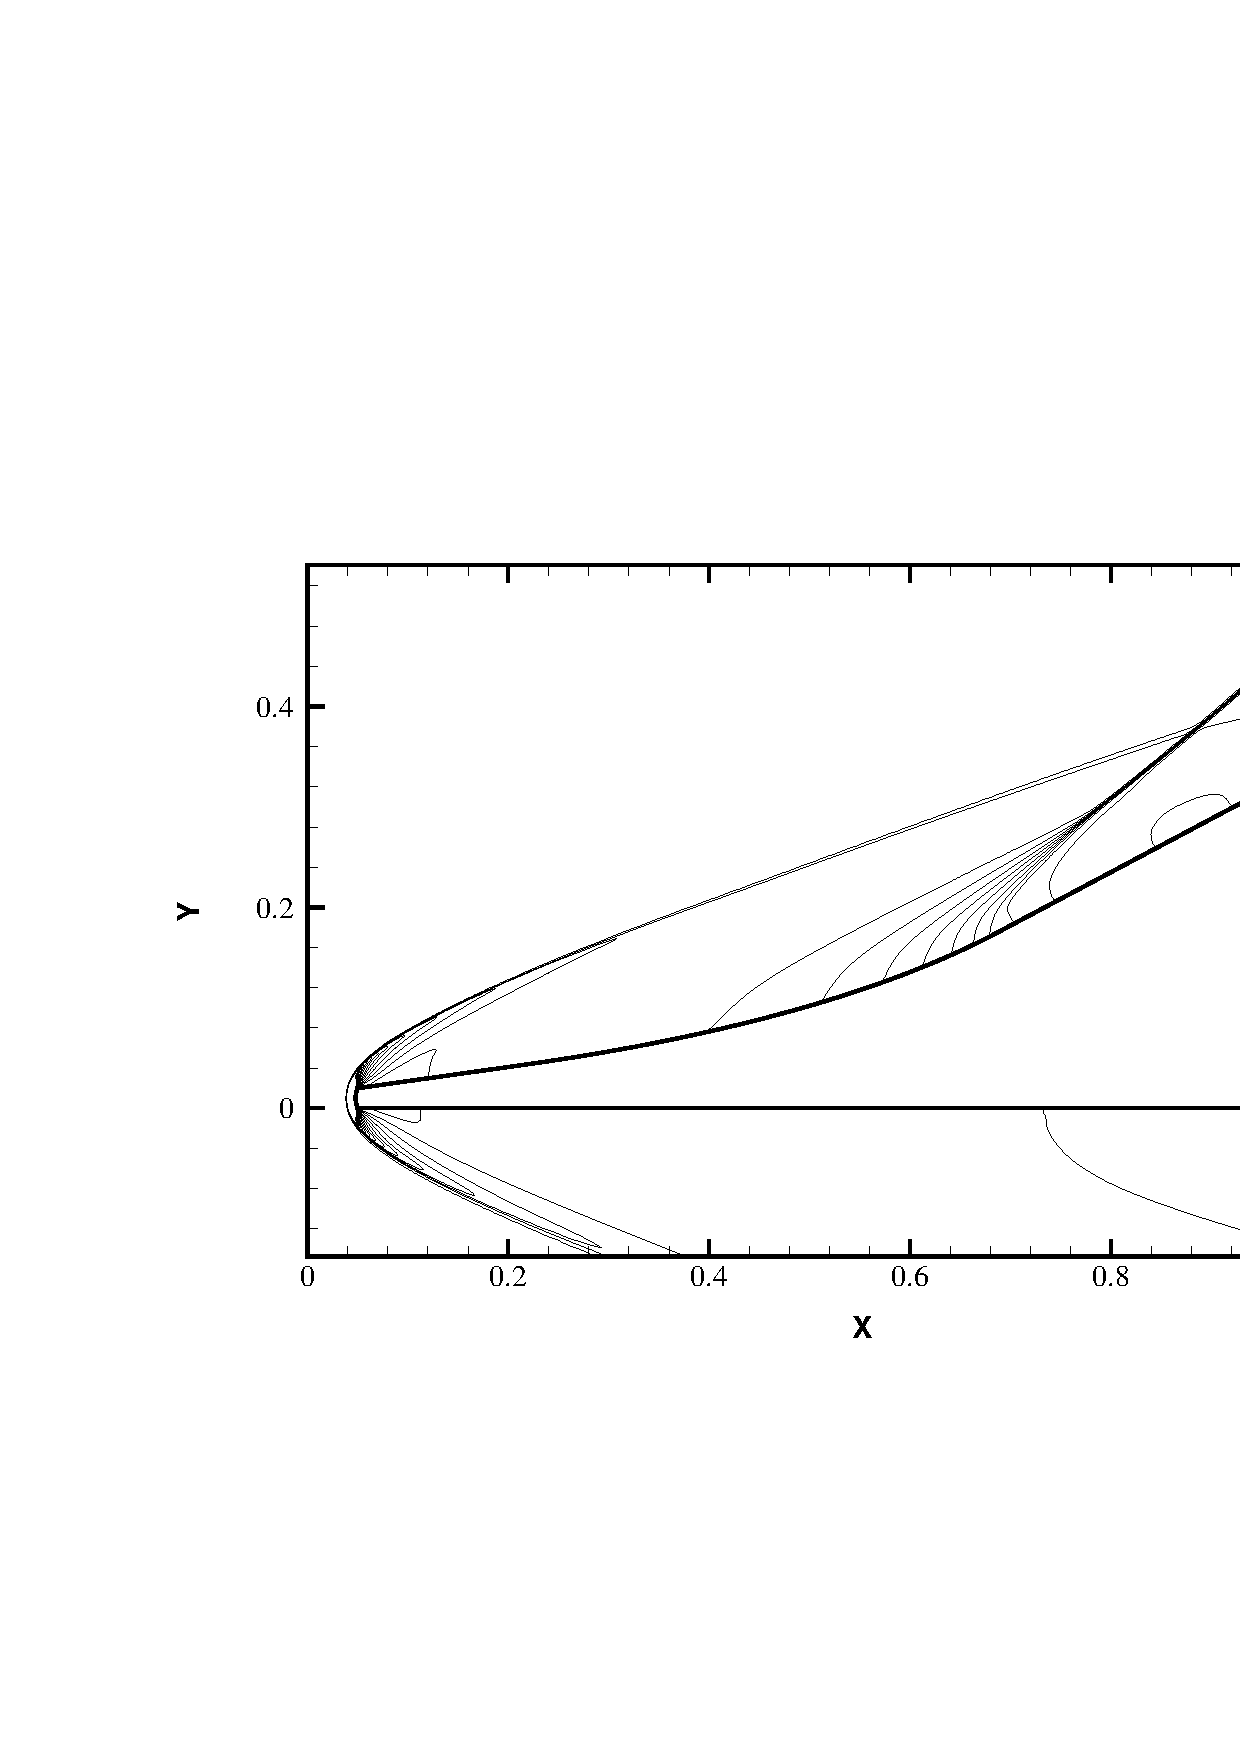
\includegraphics[width=6.3\lengthfigure]{fig3/ParentFig6.pdf}
\caption{Closeup of the pressure contours for the blunt leading edge inviscid supersonic inlet
         case obtained using a $512 \times 256$ grid;
         the inflow conditions correspond to $M=5$, $P=4$ kPa and $T=240$ K;
         no difference is noticeable between the pressure contours obtained
         with the different cycles.}
\label{fig:inlet-P}
\end{figure}
%





A first comparison between the different cycles is performed for a steady-state
inviscid flow over a 1~m long supersonic inlet. Air enters the channel at a Mach
number of 5, a pressure of 4~kPa, and a temperature of 240~K. The grid
size is varied between $128 \times 64$ nodes and $512 \times 256$
nodes. The user-defined parameters of interest are set to (when applicable)
%
\begin{displaymath}
 \sigma=0.5,~~~ \xiverge=100~\frac{1}{\rm s},~~~ \varphiverge=5000~\frac{1}{\rm s},
          ~~~\phi_0=4, ~~~ \phi_1=20, ~~~\phi_2=3, ~~~{\rm and}~~~\phi_3=9,
\end{displaymath}
%
where the value of 0.5 given to $\sigma$ translates into a geometric average
between the minimum CFL condition based pseudotime step and the maximum CFL
condition based pseudotime step. The convergence threshold $\xiverge$ is low
enough that a decrease in $\xiverge$ would not result in any noticeable
difference of the pressure contours in Figure \ref{fig:inlet-P}, except for the
active domain cycle, as pointed out later. It is noted that the use of
the entropy correction by Yee \etal\ \cite{jcp:1990:yee} with $\widetilde{\zeta}=0.2$
is here used to avoid a carbuncle
phenomenon near the shock formed by the blunt leading edge.

Table \ref{tab:inlet} shows the CPU time and effective
iterations needed to reach convergence for the marching window,
marching window / multizone, active domain, multizone, and
standard cycles. Due to the $\CFL=1$ restriction  on the traveling speed
of the waves in the flowfield to approximately one grid line per iteration,
the standard cycle requires a number of iterations proportional to the
number of grid lines along the streamwise direction, \ie\ 293 iterations
for a $128 \times 64$ mesh to 1391 iterations for a $512 \times 256$ mesh. The multizone
cycle suffers the same symptoms but has the extra advantage of \emph{not} allocating
work to the zones where all nodes exhibit a $\xi$ smaller than the user
specified threshold, therefore reducing the computing to a smaller and smaller domain
as the iteration count progresses and the non-converged flow region moves towards
the domain exit. This results in impressive savings in iteration count of
1.8 times for the coarse mesh and of 4.4 times for the fine mesh.
Both the active domain cycle and the marching window cycle decrease further the
iteration count by allowing a
computational window to travel in space following the propagation of the waves.
This results in a decrease in effective iterations, compared to the standard cycle
using the $512 \times 256$ mesh,
of 14 and 16 times for the active domain and marching window respectively.
Furthermore, the use of multizone decomposition inside the marching window
focuses the pseudotime stepping effort to the regions requiring more iterations
to reach convergence, such as the region of subsonic flow upstream of the
inlet blunt leading edge, hence resulting in only 45 effective iterations to
reach convergence and an overall reduction in effective iterations of
31 times compared to the standard cycle.
%
\begin{table}
  \fontsizetable\center
  \begin{threeparttable}
  \tablecaption{Effective iteration count, work, and storage comparison
                 for the blunt leading edge inviscid supersonic
                inlet case.\tnote{a}}
  \label{tab:inlet}
  \begin{tabular}{c@{~~~~~~}r@{.}lr@{.}lr@{.}lcr@{.}lr@{.}lr@{.}l}
    \toprule
                          &\mc{6}{c}{$128\times 64$ nodes}
                            &&\mc{6}{c}{$512\times 256$ nodes}  \\
    \cmidrule(lr){2-7}\cmidrule(lr){9-14}
    cycle                 &\mc{2}{c}{iter.}& \mc{2}{c}{work} & \mc{2}{c}{stor.}
                            &&\mc{2}{c}{iter.}& \mc{2}{c}{work} & \mc{2}{c}{stor.}\\
    \midrule
    marching window / multizone    &   34&4       &    1&0         &  0&11
                                  &&   44&9       &   22&2       &  0&91 \\

    marching window                &   40&4       &    1&1         &  0&11
                                  &&   86&8       &   38&9       &  0&91 \\

    active domain                  &   55&6       &    1&3        &  0&10
                                  &&   102&2      &   39&2       &  0&81 \\

    multizone                      &   158&5      &    3&8        &  1&0
                                  &&   318&6      &  131&6      &  16&0  \\

    standard cycle                 &   293&0      &    6&5        &  1&0
                                  &&   1391&0     &  524&3      &  16&0  \\
    \bottomrule
  \end{tabular}
  \begin{tablenotes}
    \item[a] At a CFL number of unity.
  \end{tablenotes}
  \end{threeparttable}
\end{table}
%

It is reminded that the standard cycle, the multizone cycle, and
the marching window cycle (with and without multizone decomposition)
all guarantee that
%
\begin{displaymath}
  \xi \leq \xiverge ~\forall~ {\rm inner~nodes} \, ,
\end{displaymath}
%
once convergence is reached
[as previously stated],
which is a necessary condition for a well-posed acceleration technique.
The latter is \emph{not} a property
of the active domain method when the discretization stencil for the
streamwise convection derivative depends on downstream nodes
in locally supersonic flow. The Yee TVD limiter used
here has this property, and the active domain
algorithm induces a converged residual that does not satisfy the convergence
criterion of Eq.~(...).

It could be argued that raising the CFL number would improve the standard
cycle over the others for this particular case. Investigation on a change of
CFL number is not performed, but is addressed in the subsequent test problems.
It is noted that for many realistic problems dominated by non linear phenomena,
nonlinear stability conditions restrict the use of high CFL numbers until the waves
have started to settle down considerably and for which the use
of a fine mesh results in very poor performance of the standard cycle.



  % numerical method
%% add a chapter about numerical and physical error 
%% add a chapter about the results and their analysis 
  \begin{chapterquote}
   ``(..) I realized that actually doing physics is much more enjoyable than just
   learning it. Maybe 'doing it' is the right way of learning, at least as far as
   I am concerned. ''
  \quoteauthor{Gerd Binnig, Nobel Prize Laureate in Physics, 1986}
\end{chapterquote}

\chapter{Conclusions}

\section{Numerical considerations}

A multi-species, multi-dimensional, steady-state, and time-accurate numerical method
is developed to solve the Favre-averaged Navier-Stokes equations closed by the
Wilcox $k\omega$ model. The flux discretization is based on the Yee-Roe scheme
and the pseudotime stepping on block-implicit approximate factorization.
The Wilcox $k\omega$ model along with the Wilcox dilatational dissipation
are deemed adequate in capturing the essentials of the
flowfield physics and good agreement is shown with the
experimental data of a ramp injector by Waitz {\it et al.} \cite{aiaa:1993:waitz}
and a swept ramp injector by Donohue {\it et al.} \cite{aiaa:1994:donohue}.
For a typical cantilevered ramp
injector flowfield over a flat plate, a grid refinement study is performed
and a relative error of approximately 10--15\% on the mixing efficiency is estimated
for the baseline mesh (using a grid dimensions factor $r=1$). The grid-induced
error for the three-dimensional cantilevered ramp injector flowfields is here estimated
by comparing the effect of the grid to similar two-dimensional
mixing problems where the grid can be refined sufficiently. \emph{The Richardson extrapolation
is here observed to be inadequate in determining the grid-induced error of
a mixing layer problem, due to the discontinuous turbulent/non-turbulent interface.}
The influence of the turbulent Schmidt number on the mixing
efficiency is seen to be minimal for a hydrogen-air mixing problem, as the mixing
efficiency increases by only 8\% for a turbulent Schmidt number variation from 1.0 to 0.25.
The use of the Yee entropy correction factor in conjunction with the Roe scheme
is found to be unnecessary for the inlet flowfields and its use
should be avoided as it increases significantly the numerical error in the mixing layer.


\section{Marching window acceleration technique}

Dubbed the marching window, a novel acceleration technique is presented which
is aimed at accelerating the convergence of the Favre-averaged Navier-Stokes
equations in the supersonic/hypersonic regime for flowfields with large streamwise
separated flow regions. Similarly to the active domain method \cite{aiaa:1997:nakahashi},
the marching window iterates in pseudotime a band-like computational domain of minimal
width which adjusts to the size of the streamwise elliptic regions when encountered.
However, in contrast to the active domain method, it is shown that \emph{the marching window
guarantees the residual on all nodes to be below a user-defined convergence
threshold when convergence
is reached}, and hence results in the same
converged solution (within the tolerance of the convergence criterion) as the
one obtained by standard pseudotime marching methods. Further,
a streamwise ellipticity sensor based on the Vigneron splitting
\cite{aiaaconf:1978:vigneron} is developed which ensures
the downstream boundary of the marching window to advance sufficiently
such that regions of significant streamwise
ellipticity are contained within the marching window subdomain.
It is noted that while the Vigneron splitting sensor does not capture all possible
streamwise elliptic phenomena, this does not affect the accuracy of the final solution
and only affects the performance of the marching window as an acceleration
technique. Also, a multizone decomposition is implemented inside the marching window
to restrict the computing to the zones where the residual is above the user-defined
threshold. This is shown to further decrease the work needed for convergence by close to
2 times for the test cases shown in Chapter \ref{chapter:numerical_method}.


The use of the marching window with multizone decomposition
on a backward facing step and a shock boundary
layer interaction flowfield (where one or several large streamwise separated region
is present) reveals a 4 to 6 times decrease in storage and a 4 to 8 times
decrease in work compared to the standard cycle.
The proposed algorithm is also shown to work well at
a low CFL number in regions of quasihyperbolicity/parabolicity
and is recommended for stiff
problems with high non-linear stability restrictions on the time step size.
For the inlet cases presented in Chapter ..., the marching window
with multizone decomposition results in convergence attained in typically less than
200 effective iterations using a CFL number of 0.6.
A variant of the marching window designed for time-accurate simulations
is observed to result in a fivefold reduction in storage and 25\% reduction in work
for the time-accurate exploding cavity case investigated in Chapter
\ref{chapter:numerical_method}.
The reduction in computational work through the use of the marching window
is made possible by focusing the
high number of iterations needed to converge the streamwise
separated regions to the region in question, and not to the
entire computational domain. The amount of storage needed is also significantly
reduced if no memory is allocated to the nodes outside of the marching window subdomain.


\emph{The marching window does not impose any restriction
on the discretization stencils part of the residual or on the pseudotime
stepping method.}  While not implemented here,
the numerous acceleration techniques available for pseudotime
stepping (such as multigrid, block relaxation \cite{aiaa:2000:denicola},
preconditioning, Newton-Krylov, \etc) can be used in conjunction with
the marching window.
Furthermore, the marching window is not limited to the Favre-averaged
Navier-Stokes equations and its application to other fields of physics
where a quasihyperbolicity of the system is present would only
require a redefinition of the ellipticity sensor shown in Eq.~(...).


The ellipticity threshold constant $\varphiverge$ and the marching window
minimal width $\phi_3$ are seen to affect the performance of the algorithm
significantly, and it is unclear at this stage by how much these
parameters would need to be altered for very different flow properties and physical domain size.
The dependency on the problem setup seems not too severe as the same
values for the user-specified constants are used for all inlet cases, with a resulting
similar convergence rate.



\section{Thrust potential}

The losses and the gains in the flowfields presented herein are assessed
mostly by the air-based mixing efficiency and by the thrust potential. It is
recalled that the thrust potential at a certain station corresponds
to the thrust of the vehicle obtained if the flow is reversibly expanded
from the station in consideration to either the engine exit area or the engine
back pressure.
In Chapter ..., it is shown that the thrust potential
can be expressed as a function
of the stagnation pressure, stagnation temperature, and backpressure
of the engine. While limited to a perfect gas, Eq.~(...)
shows that losses or gains in an engine cannot be determined solely by monitoring the
stagnation pressure.
This is confirmed by the inlet cases presented herein: at the station where
fuel is injected, the thrust potential increases significantly due to
the high momentum of the fuel injected while the mass flux averaged stagnation pressure
decreases. Another conclusion drawn from Eq.~(...) is that the
thrust potential can be expressed solely as a function of the stagnation temperature
and the ratio between the stagnation pressure and the backpressure. Hence, it follows
that \emph{variations
in the backpressure impact the thrust potential to the same degree as variations
in stagnation pressure}.
In a scramjet or a shcramjet engine, the flow is typically underexpanded, and
the backpressure of the engine is known to be significantly higher than the surroundings.
Expanding the flow to a fixed backpressure equal to the surroundings would hence
lead to significant errors in the thrust potential.
Therefore, the thrust potential is here determined by reversibly expanding the
flow to an iteratively determined backpressure, which is such that the cross-sectional
area of the expanded flow corresponds to the engine exit area. It is noted
that the same backpressure is shared by all streamtubes at one particular
station. In this way, we avoid errors originating
from a fixed backpressure and errors related to unrealistic
backpressure variations that would occur when expanding the flow to a constant area.
For a typical inlet flowfield, the backpressure is seen to increase by approximately
2.5 times while the mass-flux averaged stagnation pressure decreases by 4 times.
\emph{The similar observed changes in the backpressure and the stagnation
pressure shows the importance of accurately determining the backpressure when assessing
the losses in a shcramjet inlet}.

\section{Fundamental mixing studies}

%mention the conclusions from the parametric study of mixing enhancement by compression
To predict the mixing efficiency increase through a compression wave, an expression
is derived for the special case of hypersonic flow at a high convective Mach number.
In such conditions, it is seen that two assumptions can be made: (i)
the speed of the fuel and air streams
remain constant through the compression and (ii) the density increase of the air
corresponds to the density increase of the fuel through the compression. From these
two assumptions, it is then shown in the mixing efficiency growth
equation [\ie\ Eq.~(...)]
that \emph{the mixing efficiency growth is proportional to the product
of the flow density, the interface length, and the Papamoschou-Roshko correction
term.} Noting that the Papamoschou-Roshko correction term decreases for decreasing
temperature, this shows one of the major challenges of mixing in the inlet.
\emph{The very low flow density and flow temperature
lead to a very low mixing
efficiency growth in a shcramjet inlet, as compared to the mixing efficiency growth
that could be obtained in the combustor, where the temperature and the density are high.}
With the help of the derived mixing efficiency growth,
the separate effect of interface stretching due to vorticity is assessed
for a mixing layer traversing an oblique shock and a mixing layer traversing
a Prandtl-Meyer compression fan. It is observed that \emph{the higher density induced
by the compression fan leads to a greater increase in the mixing efficiency growth,
despite the more vigorous interface stretching by the axial vortices induced
by the oblique shock.}


% fundamental study of importance of ramp-induced axial vortices
The increase in mixing efficiency generally associated to ramp-like injector
configurations compared to planar mixing configurations is also analyzed.
A comparison is performed between the mixing efficiency
obtained from a planar mixing configuration, a free jet configuration
and a cantilevered ramp injector configuration.
It is seen that, at a convective Mach number of 1.5 and at a global
equivalence ratio of 1, the mixing efficiency of a cantilevered ramp injector
is as much as 4 times the one of a planar
configuration. This fourfold increase is attributed to, in order of importance:
(i) the increased fuel/air interface length present in 3D, (ii) the higher
pressure and temperature present at injection, and (iii) the stretching of the fuel/air
interface by the axial vortices.


\section{Mixing over a flat plate}

%chapter 6


A parametric study of the effect of the fuel inflow conditions on the mixing
performance of a cantilevered ramp injector  is performed.
It is found that, while keeping the fuel speed and fuel pressure constant, increasing
the global
equivalence ratio from 1 to 3 translates into a 30\% increase in the mixing efficiency,
but results in a large portion
of the mixture at the domain exit to be outside the hydrogen/air flammability limits.
On the other hand, reducing the global equivalence ratio from 1 to 0.33 reduces the mixing
efficiency by 27\%
and induces a high mixture temperature which is beneficial if burning
is desired close to the injection point, but undesirable otherwise. If burning
is not desired near the point of injection, injecting the fuel in stoichiometric
proportions with the incoming air is the recommended approach.
Secondly, keeping the global equivalence ratio and the fuel pressure constant,
the convective Mach number is varied from -0.5 to 1.5, with a negative value indicating
a fuel speed smaller than the air speed. This increase in the convective
Mach number is seen to result in a mixing efficiency increase
of 31\%  while the mass averaged stagnation pressure
decreases by only 10\%. In the near field mixing region,
the convective Mach number has a negligible impact on the mixing efficiency if using
the Wilcox dilatational dissipation. This is
shown to be related to a limitation of the turbulent mixing layer growth
due to compressibility effects occurring at a high turbulent Mach number.
Even when the convective Mach number is 0, a high turbulent Mach number is
present in the near field due to the high local shear stresses
induced by the axial vortices. Due to the presence of a high turbulent Mach number,
the dilatational dissipation reduces considerably the growth of the mixing layer.
The use of the Wilcox dilatational dissipation correction results in a decrease
of the near field mixing efficiency of 25\% and 43\% for a convective
Mach number of 0 and 1.5, respectively.
Thus, one major finding of this thesis is that \emph{the dilatational dissipation
correction affects the mixing efficiency considerably for a cantilevered
ramp injector flowfield, even at a vanishing convective Mach number.}




A parametric study of the variation of the injector array spacing shows that
the mixing efficiency at the domain exit is maximal for an array
spacing equal to the height of the injector. Reducing the spacing diminishes
considerably the axial vortices
strength but increases the interface length at the point
of injection. The rate of growth of the mixing efficiency in the nearfield is observed
to be directly related to the interface length at injection. The
decrease in the axial vortices strength at a small array spacing prevents
enough air from being entrained under the fuel jet, resulting in a
combustible mixture present in the boundary layer.
Due to the higher shock strength present above the injector array, a high angle of injection
translates into significantly more losses: injecting the fuel at 16$^\circ$
results in a twofold increase in the thrust potential losses compared to injection
at 4$^\circ$, with an associated increase in mixing efficiency
of 9\%.

A change in the fuel inflow conditions is observed not to affect the capability of
the cantilevered ramp injector at preventing the injectant from entering the
hot boundary layer. However, a change in the injector geometry
is found to result sometimes in
hydrogen entering the boundary layer. This is attributed to the amount of air separating
the fuel from the wall being strongly dependent on the injector geometry.
The reduction in the air mass flow rate separating the fuel jet from the wall
 is seen to be partly due to weakened
axial vortices and/or to a lower air mass flux flowing under the fuel at the point
of injection. It is observed that an air cushion between the wall and the
hydrogen is sufficiently thick to prevent fuel in the boundary layer
when
(i) the fuel is injected at an angle of approximately $10^\circ$ or more,
(ii) an array spacing of at least the height of the injector is used, and
(iii) a swept ramp configuration is avoided.
Another interesting finding of this thesis is that \emph{the use of a negative sweeping
angle used in conjunction with the cantilevered ramp injector configuration
is observed to result into better fuel penetration and
better mixing, and is highly recommended for mixing in a shcramjet inlet where premature
ignition should be avoided.} Lastly, it is observed that an incoming boundary layer with
a thickness of 15\% the injector height does not diminish significantly the air
cushion between the fuel and the wall.




\section{Mixing in the inlet}
%conclusions from inlet problems

Based on the results obtained from the above-mentioned parametric studies, a baseline
injector configuration is considered as a means to deliver fuel in the inlet
of an external compression shcramjet.
The baseline injector geometry consists of a sweeping angle set to the minimal
value possible, an array spacing equal to the height of the injector, and the
injection angle set to 10 degrees. Two inlet geometries are considered: one in which
the flow is compressed by two equal-strength shocks (\ie\ the shock-shock
configuration), and one in which the second shock is replaced by a Prandtl-Meyer
compression fan (\ie\ the shock-fan configuration). The fuel inflow conditions in
the inlet are such that the
global equivalence ratio approaches 1, and the convective Mach number is 1.2
with the speed of the hydrogen jet higher than the speed of the air.
\emph{Due to the fuel being injected at a very high speed, fuel injection in the inlet
is found to increase considerably the thrust potential, with a
gain exceeding the loss by 40--120\%.}
Another beneficial effect of fuel injection on the inlet performance
is the observed decrease of approximately 10\% in the skin friction force. The decrease
in skin friction is attributed to fuel being present in the boundary
layer after the second inlet compression process: the low density of
hydrogen decreases the density of the boundary layer, hence resulting
in a reduced wall shear stress. However, the presence of fuel in the inlet is not
all beneficial: due to the
Mach number of the hydrogen stream being significantly less than
the Mach number of the air stream, the performance of
the compression fan is reduced, with an associated increase in the
thrust potential losses estimated to be of 8\% for the shock-fan configurations.

\emph{Typically, it is estimated that 50--70\% of the thrust potential
losses in the inlet are due to skin friction.} The large importance of the skin friction
in the shcramjet inlet is seen to be partly due to the axial vortices generated
by the second inlet compression process continuously entraining upwards
the upper part of the boundary layer, which results in a substantial
thinning of the boundary layer, hence increasing the wall shear stress.
The use of a turbulence model that can predict accurately the wall
shear stress, such as the Wilcox $k\omega$ model used herein,
is hence seen to be crucial in assessing the losses accurately in a shcramjet
inlet. Interestingly, no recirculation region is observed near the
second inlet shock for all inlet cases studied. This is not completely
surprising, as turbulent boundary layers are known to offer a
strong resistance to separation as the flow Mach number increases \cite{jfm:1972:coleman}.
Furthermore, both the ramp-generated axial vortices and the axial vortices
generated through the second inlet shock help in reducing the size of the
boundary layer, which reduces the chance of shock-induced flow separation
in the inlet.


The relatively low mixing efficiency of 0.30 obtained for the baseline inlet
cases is attributed to the lack of adequate fuel penetration, partly
due to the absence of a sufficient amount of air separating the fuel
jets upon entering the second inlet compression process. The lack
of air in-between the fuel jets prevents the axial vortices
created by the interaction of the mixing layer with the compression fan (or shock)
to enhance fuel penetration, as they normally do by entraining the air in-between
the fuel jets to under the fuel. \emph{A major difficulty encountered while mixing in
an external compression inlet is that the height of the inlet, and hence
the amount of air entering the inlet, is strongly dependent on the fuel injection process.}
For this reason, contrarily to mixing over a flat plate,
the increase of the injection angle does not translate into a better air-based mixing
efficiency since the increase in the amount of air entering the inlet is more
pronounced than the increase in the amount of air mixed with the fuel.
\emph{One novel approach that is shown
herein to be successful at increasing the fuel penetration
is by alternating the injection angle from
one injector to another.} In this way, the fuel jets emanating from
the high-angle injectors penetrate deeply in the incoming air, while the
fuel jets emanating from the low-angle injectors remain close to the body.
Upon entering the compression process, due to the fuel jets belonging
to two distinct levels, there is a much increased amount of air separating
the fuel jets on each level and the compression process induces better
penetration. Furthermore, the strength of the shock forming on the injector array
does not increase appreciably due to one in every two injector being at a low
angle. The reduced array shock strength  helps in keeping the inlet height
to a low value. The use of alternating injection angles of 9 and 16 degrees
is seen to result in a 32\% increase in the mixing efficiency and a 14\% increase
in the thrust potential losses when compared to injecting the fuel at a single injection
angle of 10 degrees. A second strategy that is shown to increase the fuel penetration
and the mixing efficiency is the use of longer and thinner cantilevered ramp injectors.
By doubling the length of the injector, while doubling the height and halving the depth
of the fuel
jet, a mixing efficiency increase of 15\% is observed at the expense of an increase
in thrust potential losses of 12\%. The combination of the alternating angle
configuration with the longer and thinner injectors results in a mixing efficiency
of 0.47 and 0.44 for the shock-shock inlet configuration and the shock-fan inlet
configuration respectively, which is an increase of more than 50\% over the baseline
injector configuration.


% risk of premature ignition
Premature ignition in the inlet is a high possibility for the baseline inlet
configurations, as a fuel/air mixture is seen to penetrate the
hot boundary layer after the second inlet compression wave. One strategy that is
here shown to prevent to a large extent the fuel
from entering the boundary layer is the use of an increased injector array spacing.
A higher array spacing increases the amount of air that is entrained by the axial vortices
below the fuel jets, hence retarding the complete erosion of the air buffer separating
the fuel from the wall. Unfortunately,
while a higher array spacing prevents the fuel from entering the boundary layer,
it results in stronger axial vortices which entrain upwards the hot flow from the
boundary layer to the mixing layer. This is particularly worrisome as the mixing
layer is then exposed to a temperature significantly above the ignition
point for a considerable amount of time, resulting in a high risk of premature ignition.
Nonetheless, the risk of premature ignition in the mixing layer can be reduced
through the use of a shock-fan configuration, which results in
a reduction in the flow temperature of as much as 80~K compared to the
shock-shock configuration. Besides helping to prevent the risk of premature ignition,
a reduction of the temperature of the flow entering the combustor augments the
performance of the shcramjet due to a
more efficient heat released in the shock-induced combustion \cite{jpp:2001:sislian}.
\emph{The use of a Prandtl-Meyer compression surface in a shcramjet inlet is hence strongly
recommended as it decreases the thrust potential losses, reduces
the risk of premature ignition, while resulting in a small 6\% diminution of the
mixing efficiency for the optimal injector configuration considered.}


  % conclusions

  %%%%%%%=--appendix--=%%%%%%%
  \appendix
  \chapter{Test Appendix}

%
\begin{equation}
a=b+c
\end{equation}
%


  %%%%%%%=--bibliography--=%%%%%%%
  % the next line is to cite papers that may are not cited in the text
  \nocite{jcp:2002:parent,aiaaconf:2001:parent,aiaa:2002:parent,aiaa:2003:parent,aiaa:2003:parent:2,
          jpp:2003:sislian,aiaaconf:2002:sislian}
  \bibliographystyle{waflthesis}
  \bibliography{aiaa,jpp,jfm,jcp,nasa,cf,misc,book,thesis,vki}

\end{document}

